\chapter{Âmbito do Produto}
\section{Diagrama de \textit{Use Cases}}
De maneira a compreender melhor o contexto do sistema, vai ser apresentado um diagrama de \textit{Use Cases}. Neste vão ser explicitadas algumas das principais funcionalidades do sistema, bem como os atores do mesmo.
Neste diagrama, é ainda possível identificar, quais as funcionalidades a que cada tipo de ator do sistema vai ter acesso.

\begin{figure}[H]
\centering
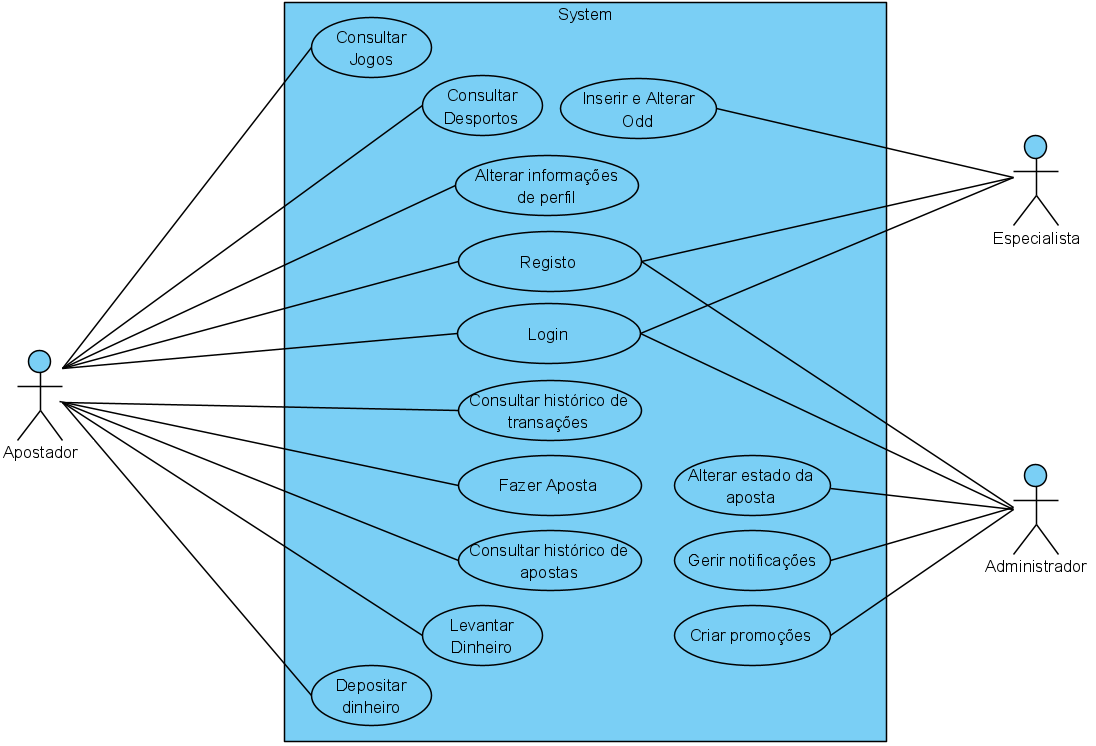
\includegraphics[width=1\textwidth]{imagens/ambitoProduto/Casos_de_uso_NEW.png}
\caption{Diagrama de \textit{Use Cases}}
\end{figure}
\newpage
\section{Atores}
Como está representado no diagrama anterior, o nosso sistema suporta dois tipos de atores: o Apostador e o Especialista. 
\par
O \textbf{Apostador} é o utilizador comum do nosso sistema, vai ter acesso a todas as funcionalidades que a nossa plataforma oferece ao público. 
\par 
O \textbf{Especialista} é o indivíduo que ajustará as \textit{odds} para os futuros jogos, e por isso, para além dessa, as únicas funcionalidades que lhe estão disponíveis são o registo e login.

O \textbf{Administrador} é o indivíduo responsável pela gestão do estado da aposta (suspensa, fechada, ativa), pela gestão das notificações, pela criação de promoções, e por isso, para além dessas, as únicas funcionalidades que lhe estão disponíveis são o registo e login.

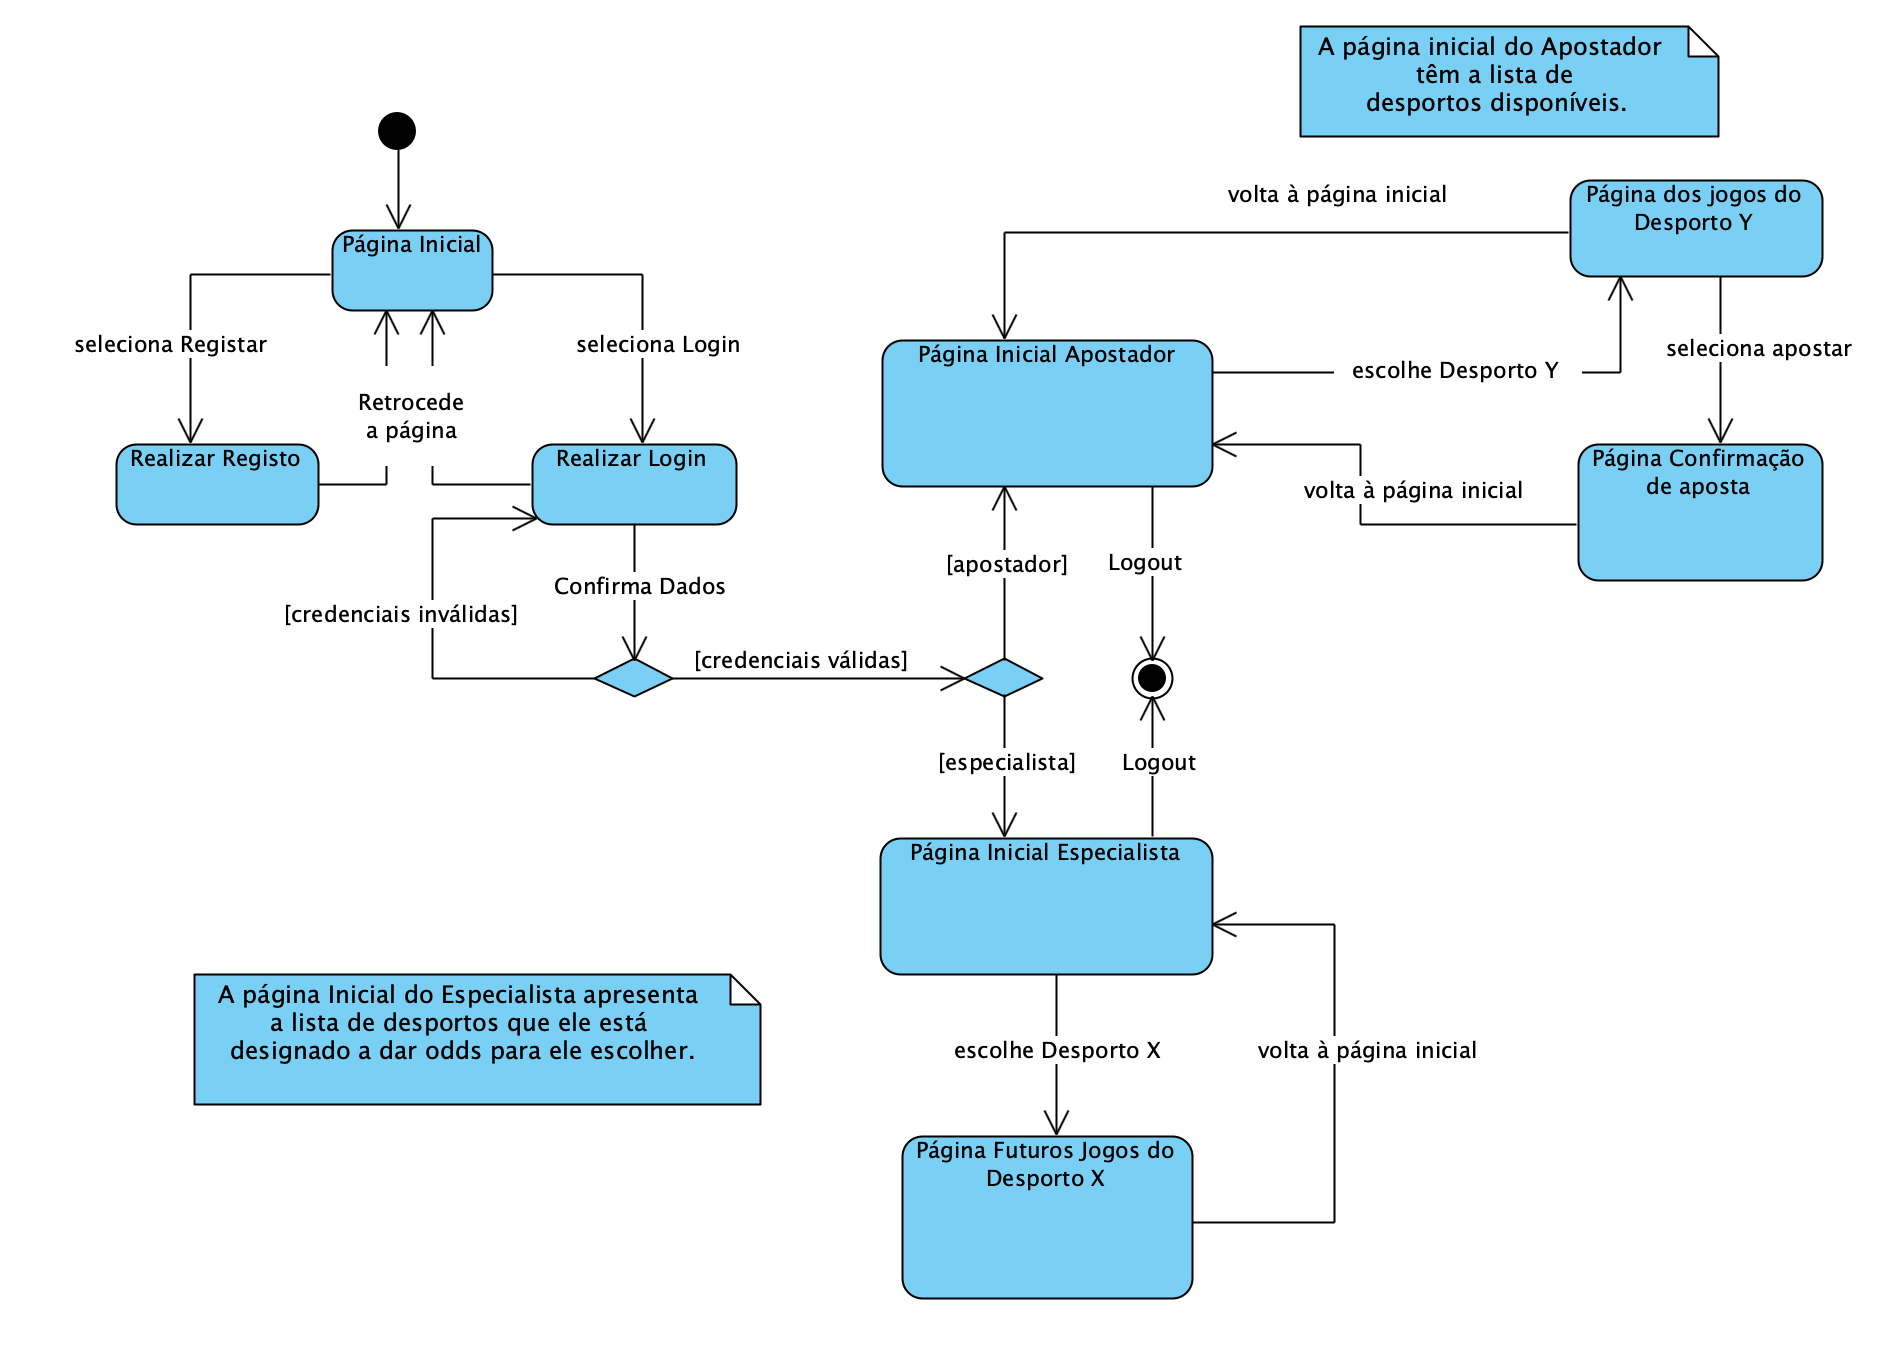
\includegraphics[width=1\textwidth]{imagens/ambitoProduto/maqEstados.png}


\section{Breve Descrição dos Use Cases}
Nesta secção será apresentada uma especificação tabelar de cada \textit{Use Case} considerado, de modo a facilitar todo o processo de implementação de cada funcionalidade do nosso sistema.\\
Deste modo, consideramos que é bastante perceptível o fluxo sequencial da interacção do ator com o sistema.

\subsection{Registar Apostador}
O \textit{use case} Registar para o ator Apostador consiste no registo de um apostador, que ainda não se encontra no sistema.\\
Os casos de erro acontecem quando o sistema deteta uma tentativa de inserir um apostador que já se encontra registado ou caso a \textit{password} pretendida não cumpra os requisitos impostos pelo grupo de uma \textit{password} válida.

\begin{table}[H]
\begin{center}
\scalebox{0.70}{
\begin{tabular}{|l|l|l|}
\hline
\textbf{USE-CASE:} & \multicolumn{2}{l|}{Registar} \\ \hline
\textbf{Ator:} & \multicolumn{2}{l|}{apostador} \\ \hline
\textbf{Pré-Condição:} & \multicolumn{2}{l|}{Ator não está registado no sistema} \\ \hline
\textbf{Pós-Condição:} & \multicolumn{2}{l|}{Ator está registado} \\ \hline
%\multirow 
{\textbf{Cenário Normal}} & \textbf{Ator Input} & \textbf{System Response} \\ \cline{2-3}
& 2 - Fornece credenciais. & \begin{tabular}[c]{@{}l@{}}1- Pede credenciais de  acesso.\\ \\ \\ \\ 3 - Valida credenciais.\\ 4 - Informa que o apostador está registado.\end{tabular} \\ \hline
\begin{tabular}[c]{@{}l@{}}\textbf{Exceção 1 :} {[}username existente{]}\\ (Passo 3)\end{tabular} &  & \begin{tabular}[c]{@{}l@{}}3.1 - Informa o apostador que o username já \\ existe no sistema.\end{tabular} \\ \hline
\begin{tabular}[c]{@{}l@{}}\textbf{Exceção 2 :} {[}password inválida{]}\\  (passo 3)\end{tabular} &  & \begin{tabular}[c]{@{}l@{}}3.2 - Informa o apostador que a password não cumpre\\ os requisitos necessários.\end{tabular} \\ \hline
\end{tabular}}
\caption{Especificação de \textit{Use Case} Registar Apostador}
\end{center}
\end{table}

\newpage
\subsection{Login Apostador}
O \textit{use case} Login Apostador consiste na autenticação de um apostador que se encontra no sistema, sendo o seu login feito através dos seguintes parâmetros : email e \textit{password}.
Os casos de erro acontecem quando o sistema deteta uma tentativa de autenticar um apostador que não se encontra registado ou caso a \textit{password} do apostador não seja correspondente com a que existe no sistema.
\begin{table}[H]
\begin{center}
\scalebox{0.80}{
\begin{tabular}{|p{50mm}|p{40mm}|p{80mm}|}
\hline
\textbf{USE-CASE:} & \multicolumn{2}{l|}{Login} \\ \hline
\textbf{Ator:} & \multicolumn{2}{l|}{Apostador} \\ \hline
\textbf{Pré-Condição:} & \multicolumn{2}{l|}{Ator não está autenticado} \\ \hline
\textbf{Pós-Condição:} & \multicolumn{2}{l|}{Ator está autenticado} \\ \hline
%\multirow
{\textbf{Cenário Normal}} & \textbf{Ator Input} & \textbf{System Response} \\ \cline{2-3}
& 2 - Fornece credenciais. & \begin{tabular}[c]{@{}l@{}}1- Pede credenciais de acesso.\\ \\ 3 - Valida credenciais.\\ 4 - Informa que o apostador está autenticado.\end{tabular} \\ \hline
\begin{tabular}[c]{@{}l@{}}\textbf{Alternativa 1 :}  \\{[}password incorreta{]}\\  (passo 3)\end{tabular} &  & \begin{tabular}[c]{@{}l@{}}3.1 - Informa o apostador que a password \\ não corresponde ao email fornecido. \\3.2- Voltar ao passo 2 \end{tabular} \\ \hline
\begin{tabular}[c]{@{}l@{}}\textbf{Exceção 1 :}\\ {[}email inexistente]\\ (Passo 3){]}\end{tabular} &  & \begin{tabular}[c]{@{}l@{}}3.1.1 - Informa o apostador que o email \\ não existe no sistema.\end{tabular} \\ \hline
\end{tabular}}
\end{center}
\caption{Especificação de \textit{Use Case} Login Apostador}
\end{table}

\subsection{Login Especialista}
O \textit{use case} Login Especialista consiste na autenticação de um especialista com credenciais de acesso para entrar no sistema, sendo o seu login feito através dos seguintes parâmetros : email e \textit{password}.
Os casos de erro acontecem quando o sistema deteta uma tentativa de autenticar um especialista cujo o email não consta no sistema ou caso a \textit{password} do especialista não seja correspondente com a que existe no sistema.
\begin{table}[H]
\begin{center}
\scalebox{0.80}{
\begin{tabular}{|p{50mm}|p{40mm}|p{80mm}|}
\hline
\textbf{USE-CASE:} & \multicolumn{2}{l|}{Login} \\ \hline
\textbf{Ator:} & \multicolumn{2}{l|}{Especialista} \\ \hline
\textbf{Pré-Condição:} & \multicolumn{2}{l|}{Ator não está autenticado} \\ \hline
\textbf{Pós-Condição:} & \multicolumn{2}{l|}{Ator está autenticado} \\ \hline
%\multirow
{\textbf{Cenário Normal}} & \textbf{Ator Input} & \textbf{System Response} \\ \cline{2-3}
& 2 - Fornece credenciais. & \begin{tabular}[c]{@{}l@{}}1- Pede credenciais de acesso.\\ \\ 3 - Valida credenciais.\\ 4 - Informa que o especialista está autenticado.\end{tabular} \\ \hline
\begin{tabular}[c]{@{}l@{}}\textbf{Alternativa 1 :}  \\{[}password incorreta{]}\\  (passo 3)\end{tabular} &  & \begin{tabular}[c]{@{}l@{}}3.1 - Informa o especialista que a password \\ não corresponde ao email fornecido. \\3.2- Voltar ao passo 2 \end{tabular} \\ \hline
\begin{tabular}[c]{@{}l@{}}\textbf{Exceção 1 :}\\ {[}email inexistente]\\ (Passo 3)\end{tabular} &  & \begin{tabular}[c]{@{}l@{}}3.1.1 - Informa o especialista que o email \\ não existe no sistema.\end{tabular} \\ \hline
\end{tabular}}
\end{center}
\caption{Especificação de \textit{Use Case} Login Especialista}
\end{table}

\newpage
\subsection{Login Administrador}
O \textit{use case} Login Administrador consiste na autenticação de um administrador com credenciais de acesso para entrar no sistema, sendo o seu login feito através dos seguintes parâmetros : email e \textit{password}.
Os casos de erro acontecem quando o sistema deteta uma tentativa de autenticar um administrador cujo o email não consta no sistema ou caso a \textit{password} do especialista não seja correspondente com a que existe no sistema.
\begin{table}[H]
\begin{center}
\scalebox{0.80}{
\begin{tabular}{|p{50mm}|p{40mm}|p{80mm}|}
\hline
\textbf{USE-CASE:} & \multicolumn{2}{l|}{Login} \\ \hline
\textbf{Ator:} & \multicolumn{2}{l|}{Especialista} \\ \hline
\textbf{Pré-Condição:} & \multicolumn{2}{l|}{Ator não está autenticado} \\ \hline
\textbf{Pós-Condição:} & \multicolumn{2}{l|}{Ator está autenticado} \\ \hline
%\multirow
{\textbf{Cenário Normal}} & \textbf{Ator Input} & \textbf{System Response} \\ \cline{2-3}
& 2 - Fornece credenciais. & \begin{tabular}[c]{@{}l@{}}1- Pede credenciais de acesso.\\ \\ 3 - Valida credenciais.\\ 4 - Informa que o administrador está autenticado.\end{tabular} \\ \hline
\begin{tabular}[c]{@{}l@{}}\textbf{Alternativa 1 :}  \\{[}password incorreta{]}\\  (passo 3)\end{tabular} &  & \begin{tabular}[c]{@{}l@{}}3.1 - Informa o administrador que a password \\ não corresponde ao email fornecido. \\3.2- Voltar ao passo 2 \end{tabular} \\ \hline
\begin{tabular}[c]{@{}l@{}}\textbf{Exceção 1 :}\\ {[}email inexistente]\\ (Passo 3)\end{tabular} &  & \begin{tabular}[c]{@{}l@{}}3.1.1 - Informa o administrador que o email \\ não existe no sistema.\end{tabular} \\ \hline
\end{tabular}}
\end{center}
\caption{Especificação de \textit{Use Case} Login Administrador}
\end{table}

\newpage
\subsection{Alterar informações de perfil}
O \textit{use case} Alterar informações de perfil consiste no apostador alterar os parâmetros editáveis do seu perfil, que são o nome e o email (cenário normal). Caso este pretenda alterar a morada ou o número de telemóvel, só o poderá fazer com passos adicionais "mais seguros", para confirmar a sua identidade, como por exemplo, receber uma mensagem com um código para proceder à sua alteração (cenário adicional). Dados mais "sensíveis" como Nº de Identificação Fiscal, Nº do Cartão de cidadão e Data de Nascimento não são editáveis.
\begin{table}[H]
\begin{center}
\scalebox{0.80}{
\begin{tabular}{|p{40mm}|p{50mm}|p{80mm}|}
\hline
\textbf{USE-CASE:} & \multicolumn{2}{l|}{Alterar informações de perfil} \\ \hline
\textbf{Ator:} & \multicolumn{2}{l|}{Apostador} \\ \hline
\textbf{Pré-Condição:} & \multicolumn{2}{l|}{Ator autenticado} \\ \hline
\textbf{Pós-Condição:} & \multicolumn{2}{l|}{Ator contém informações de perfil editadas} \\ \hline
%\multirow
{\textbf{Cenário Normal}} & \textbf{Ator Input} & \textbf{System Response} \\ \cline{2-3}
& \begin{tabular}[c]{@{}l@{}} 1 - Informa o sistema que \\ pretende editar as suas\\ informações. \\ \\  3- Altera informações. \\ 4 - Guarda alterações.  \end{tabular}&  \begin{tabular}[c]{@{}l@{}} \\ \\ \\2 - Apresenta campos de informação em modo \\de edição.\\ \\ \\ \\5 - Informa que as alterações foram guardadas.\end{tabular} \\ \hline
%\multirow
{\textbf{Cenário Adicional}} & \textbf{Ator Input} & \textbf{System Response} \\ \cline{2-3}
& \begin{tabular}[c]{@{}l@{}} 1 - Informa o sistema que \\ pretende editar as suas\\ informações. \\ 3 - Preenche o campo com o \\que é pedido. \\ 5 - Coloca o código no campo. \\ 7 - Altera as informações. \\ 8 - Guarda as alterações. \end{tabular}&  \begin{tabular}[c]{@{}l@{}} 2 - Apresenta um campo para que o utilizador\\insira o número de telemóvel.\\ 4 - O sistema envia um código para o \\ respetivo número. \\6 - Apresenta campos de informação em \\ modo de edição. \\ 9 - Informa que as alterações foram guardadas. \end{tabular} \\ \hline
\end{tabular}}
\end{center}
\caption{Especificação de \textit{Use Case} Alterar informações de perfil}
\end{table}

\subsection{Consultar jogos}
O \textit{use case} Consultar jogos permite ao utilizador selecionar um ou mais desportos e ver a lista de jogos desse(s) desporto(s).
\begin{table}[H]
\begin{center}
\scalebox{0.80}{
\begin{tabular}{|p{40mm}|p{70mm}|p{80mm}|}
\hline
\textbf{USE-CASE:} & \multicolumn{2}{l|}{Consultar jogos} \\ \hline
\textbf{Ator:} & \multicolumn{2}{l|}{Apostador} \\ \hline
\textbf{Pré-Condição:} & \multicolumn{2}{l|}{Ator autenticado} \\ \hline
\textbf{Pós-Condição:} & \multicolumn{2}{l|}{Ator acede a uma lista de jogos} \\ \hline
%\multirow
{\textbf{Cenário Normal}} & \textbf{Ator Input} & \textbf{System Response} \\ \cline{2-3}
& \begin{tabular}[c]{@{}l@{}} 1 - Informa o sistema qual o desporto\\ que pretende consultar.   \end{tabular}&  \begin{tabular}[c]{@{}l@{}}\\ \\ \\ \\2 - Apresenta a lista de jogos desse desporto.\end{tabular} \\ \hline
\end{tabular}}
\end{center}
\caption{Especificação de\textit{ Use Case} Consultar jogos}
\end{table}

\newpage
\subsection{Fazer aposta}
O \textit{use case} Fazer aposta consiste no utilizador selecionar um resultado de jogo, escolher a quantia a apostar e efetuar o pagamento da mesma.
\begin{table}[H]
\begin{center}
\scalebox{0.80}{
\begin{tabular}{|p{40mm}|p{50mm}|p{80mm}|}
\hline
\textbf{USE-CASE:} & \multicolumn{2}{l|}{Consultar jogos} \\ \hline
\textbf{Ator:} & \multicolumn{2}{l|}{Apostador} \\ \hline
\textbf{Pré-Condição:} & \multicolumn{2}{l|}{Ator autenticado} \\ \hline
\textbf{Pós-Condição:} & \multicolumn{2}{l|}{Ator obtém confirmação de aposta} \\ \hline
%\multirow
{\textbf{Cenário Normal}} & \textbf{Ator Input} & \textbf{System Response} \\ \cline{2-3}
& \begin{tabular}[c]{@{}l@{}} 1 - Informa o sistema qual o \\ jogo e montante que pretende\\ apostar. \\ 2 - Confirma aposta. \\ \\ \\ 4 - Realiza pagamento. \end{tabular}&  \vspace{3.5mm} \begin{tabular}[c]{@{}l@{}} 3 - Solicita pagamento da \\ aposta. \\ \\ 5 - Valida o pagamento. \\ 6- Informa o apostador que a aposta foi \\ realizada com sucesso.\end{tabular} \\ \hline
\begin{tabular}[c]{@{}l@{}}\textbf{Exceção 1 :}\\ {[}método de pagamento \\ inválido]\\ (Passo 5)\end{tabular} &  & \begin{tabular}[c]{@{}l@{}}5.1 - Informa o apostador que o método de \\ pagamento usado não é válido. \\ 5.2 - Volta ao passo 4. \end{tabular} \\ \hline
\end{tabular}}
\end{center}
\caption{Especificação de \textit{Use Case} Fazer aposta}
\end{table}

\subsection{Consultar histórico de apostas}
O \textit{use case} Consultar histórico de apostas consiste em apresentar ao apostador a lista de apostas que ele já realizou no sistema.
\begin{table}[H]
\begin{center}
\scalebox{0.80}{
\begin{tabular}{|p{40mm}|p{60mm}|p{70mm}|}
\hline
\textbf{USE-CASE:} & \multicolumn{2}{l|}{Consultar histórico de apostas} \\ \hline
\textbf{Ator:} & \multicolumn{2}{l|}{Apostador} \\ \hline
\textbf{Pré-Condição:} & \multicolumn{2}{l|}{Ator autenticado} \\ \hline
\textbf{Pós-Condição:} & \multicolumn{2}{l|}{Ator obtém a lista de apostas já realizadas} \\ \hline
%\multirow
{\textbf{Cenário Normal}} & \textbf{Ator Input} & \textbf{System Response} \\ \cline{2-3}
& \begin{tabular}[c]{@{}l@{}} 1 - Informa o sistema a intenção \\ de ver o seu histórico de apostas. \end{tabular} &  \begin{tabular}[c]{@{}l@{}} \\ \\ \\2 - Apresenta a lista de apostas \\ já realizadas pelo apostador.\end{tabular} \\ \hline
\end{tabular}}
\end{center}
\caption{Especificação de \textit{Use Case} Consultar histórico de apostas}
\end{table}

\newpage
\subsection{Consultar histórico de transações}
O \textit{use case} Consultar histórico de transações consiste em apresentar ao apostador os movimentos de dinheiro da sua conta tais como depósitos, levantamentos, ganhos e perdas de apostas.
\begin{table}[H]
\begin{center}
\scalebox{0.80}{
\begin{tabular}{|p{40mm}|p{60mm}|p{70mm}|}
\hline
\textbf{USE-CASE:} & \multicolumn{2}{l|}{Consultar histórico de transações} \\ \hline
\textbf{Ator:} & \multicolumn{2}{l|}{Apostador} \\ \hline
\textbf{Pré-Condição:} & \multicolumn{2}{l|}{Ator autenticado} \\ \hline
\textbf{Pós-Condição:} & \multicolumn{2}{l|}{Ator obtém uma lista de movimentos de conta} \\ \hline
%\multirow
{\textbf{Cenário Normal}} & \textbf{Ator Input} & \textbf{System Response} \\ \cline{2-3}
& \begin{tabular}[c]{@{}l@{}} 1 - Informa o sistema a intenção \\ de ver o seu histórico de transações. \end{tabular} &  \begin{tabular}[c]{@{}l@{}} \\ \\ \\2 - Apresenta a lista de movimentos \\ do apostador.\end{tabular} \\ \hline
\end{tabular}}
\end{center}
\caption{Especificação de \textit{Use Case} Consultar histórico de transações}
\end{table}

\subsection{Depositar dinheiro}
O \textit{use case} Depositar dinheiro consiste na intenção do apostador em adicionar dinheiro ao seu saldo.
\begin{table}[H]
\begin{center}
\scalebox{0.80}{
\begin{tabular}{|p{40mm}|p{55mm}|p{75mm}|}
\hline
\textbf{USE-CASE:} & \multicolumn{2}{l|}{Depositar dinheiro} \\ \hline
\textbf{Ator:} & \multicolumn{2}{l|}{Apostador} \\ \hline
\textbf{Pré-Condição:} & \multicolumn{2}{l|}{Ator autenticado} \\ \hline
\textbf{Pós-Condição:} & \multicolumn{2}{l|}{Ator com mais dinheiro na sua conta} \\ \hline
%\multirow
{\textbf{Cenário Normal}} & \textbf{Ator Input} & \textbf{System Response} \\ \cline{2-3}
& \begin{tabular}[c]{@{}l@{}} 1 - Informa o sistema a intenção \\ de depositar dinheiro. \\ \\ 3 - Realiza transferência. \end{tabular} &  \begin{tabular}[c]{@{}l@{}} \\ \\ \\ \\ \\ 2 - Solicita a escolha do montante \\ e forma de transferência. \\ \\ 4 - Valida transferência. \\ 5 -  Informa o apostador que a transferência \\  foi realizada com sucesso.\end{tabular} \\ \hline
\begin{tabular}[c]{@{}l@{}}\textbf{Exceção 1 :}\\ {[}método de pagamento \\ inválido]\\ (Passo 4)\end{tabular} &  & \begin{tabular}[c]{@{}l@{}}4.1 - Informa o apostador que o método de \\ transferência usado não é válido. \\ 4.2 - Volta ao passo 3. \end{tabular} \\ \hline
\end{tabular}}
\end{center}
\caption{Especificação de \textit{Use Case} Depositar dinheiro}
\end{table}

\newpage
\subsection{Levantar dinheiro}
O \textit{use case} Levantar dinheiro consiste na intenção do apostador em levantar dinheiro da sua conta.
\begin{table}[H]
\begin{center}
\scalebox{0.80}{
\begin{tabular}{|p{40mm}|p{55mm}|p{75mm}|}
\hline
\textbf{USE-CASE:} & \multicolumn{2}{l|}{Levantar dinheiro} \\ \hline
\textbf{Ator:} & \multicolumn{2}{l|}{Apostador} \\ \hline
\textbf{Pré-Condição:} & \multicolumn{2}{l|}{Ator autenticado e com saldo positivo na conta} \\ \hline
\textbf{Pós-Condição:} & \multicolumn{2}{l|}{Ator com menos dinheiro na sua conta} \\ \hline
%\multirow
{\textbf{Cenário Normal}} & \textbf{Ator Input} & \textbf{System Response} \\ \cline{2-3}
& \begin{tabular}[c]{@{}l@{}} 1 - Informa o sistema a intenção \\ de levantar dinheiro. \\ \\ 3 - Realiza transferência. \end{tabular} &  \begin{tabular}[c]{@{}l@{}} \\ \\ \\ \\ \\ 2 - Solicita a escolha do montante \\ e forma de transferência. \\ \\ 4 - Valida transferência. \\ 5 -  Informa o apostador que a transferência \\  foi realizada com sucesso.\end{tabular} \\ \hline
\begin{tabular}[c]{@{}l@{}}\textbf{Exceção 1 :}\\ {[}método de pagamento \\ inválido]\\ (Passo 4)\end{tabular} &  & \begin{tabular}[c]{@{}l@{}}4.1 - Informa o apostador que o método de \\ transferência usado não é válido. \\ 4.2 - Volta ao passo 3. \end{tabular} \\ \hline
\end{tabular}}
\end{center}
\caption{Especificação de \textit{Use Case} Levantar dinheiro}
\end{table}

\subsection{Inserir \textit{odd}}
O \textit{use case} Inserir \textit{odd} apenas está disponível para o Especialista e consiste neste fixar a \textit{odd} de jogos futuros.
\begin{table}[H]
\begin{center}
\scalebox{0.80}{
\begin{tabular}{|p{40mm}|p{60mm}|p{70mm}|}
\hline
\textbf{USE-CASE:} & \multicolumn{2}{l|}{Inserir odd} \\ \hline
\textbf{Ator:} & \multicolumn{2}{l|}{Especialista} \\ \hline
\textbf{Pré-Condição:} & \multicolumn{2}{l|}{Ator autenticado} \\ \hline
\textbf{Pós-Condição:} & \multicolumn{2}{l|}{Odds de jogo(s) futuros definida(s)} \\ \hline
%\multirow
{\textbf{Cenário Normal}} & \textbf{Ator Input} & \textbf{System Response} \\ \cline{2-3}
& \begin{tabular}[c]{@{}l@{}} 1 - Escolhe um desporto. \\ \\ \\ 3 - Fixa odd para um ou mais jogos. \\ 4 - Guarda alterações. \end{tabular} &  \begin{tabular}[c]{@{}l@{}} \\ 2 - Apresenta a lista de jogos sem odds \\ do desporto escolhido. \\ \\ \\ 5 - Informa o especialista que as odds \\ foram guardadas com sucesso.\end{tabular} \\ \hline
\end{tabular}}
\end{center}
\caption{Especificação de \textit{Use Case} Inserir \textit{odd}}
\end{table}

\newpage
\subsection{Alterar estado da aposta}
O \textit{use case} Alterar estado da aposta apenas está disponível para o Administrador e consiste neste alterar o estado da aposta (ativa, fechada ou suspensa), no caso de, por exemplo, acontecer alguma situação que leve à sua suspensão.
\begin{table}[H]
\begin{center}
\scalebox{0.80}{
\begin{tabular}{|p{40mm}|p{60mm}|p{70mm}|}
\hline
\textbf{USE-CASE:} & \multicolumn{2}{l|}{Alterar estado da aposta} \\ \hline
\textbf{Ator:} & \multicolumn{2}{l|}{Administrador} \\ \hline
\textbf{Pré-Condição:} & \multicolumn{2}{l|}{Administrador autenticado} \\ \hline
\textbf{Pós-Condição:} & \multicolumn{2}{l|}{Estado da aposta alterado} \\ \hline
%\multirow
{\textbf{Cenário Normal}} & \textbf{Ator Input} & \textbf{System Response} \\ \cline{2-3}
& \begin{tabular}[c]{@{}l@{}} 1 - Informa o sistema a vontade de \\ alterar o estado da aposta. \\ 2 - Ativa, fecha ou suspende a aposta. \\ 3 - Guarda as alterações feitas. \end{tabular} &  \vspace{5mm} \begin{tabular}[c]{@{}l@{}}  4 - Informa o administrador que a operação \\ foi efetuada com sucesso.\end{tabular} \\ \hline
\end{tabular}}
\end{center}
\caption{Especificação de \textit{Use Case} Alterar estado da aposta}
\end{table}

\newpage
\section{Diagramas de Sequência e Mockups}
Os Diagramas de Sequência são Diagramas de Interação cujo foco é, principalmente, a ordenação temporal das mensagens e representação das mesmas.
Desta forma, tendo por base o nosso Diagrama de Classes, desenvolvemos os seguintes Diagramas de Sequência representativos do funcionamento do sistema.

\subsection{Registo Apostador}
\begin{figure}[H]
\centering
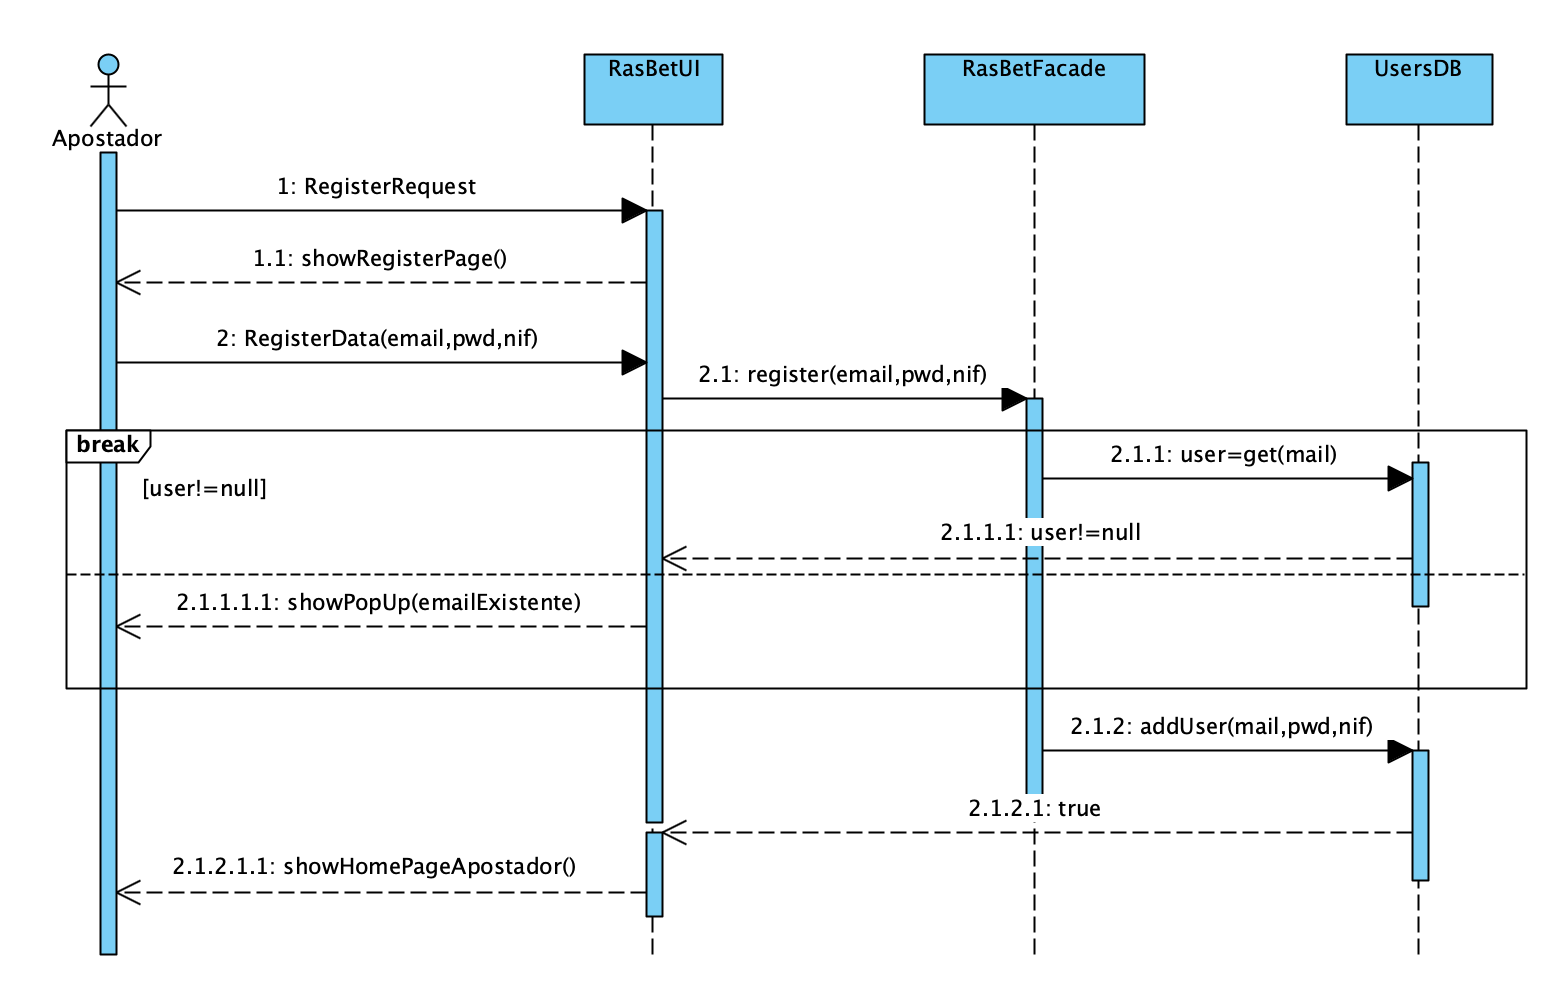
\includegraphics[width=0.8\textwidth]{imagens/ambitoProduto/SRegisto.png}
\caption{Diagrama de Sequência de Registo}
\end{figure}
\begin{figure}[H]
\centering
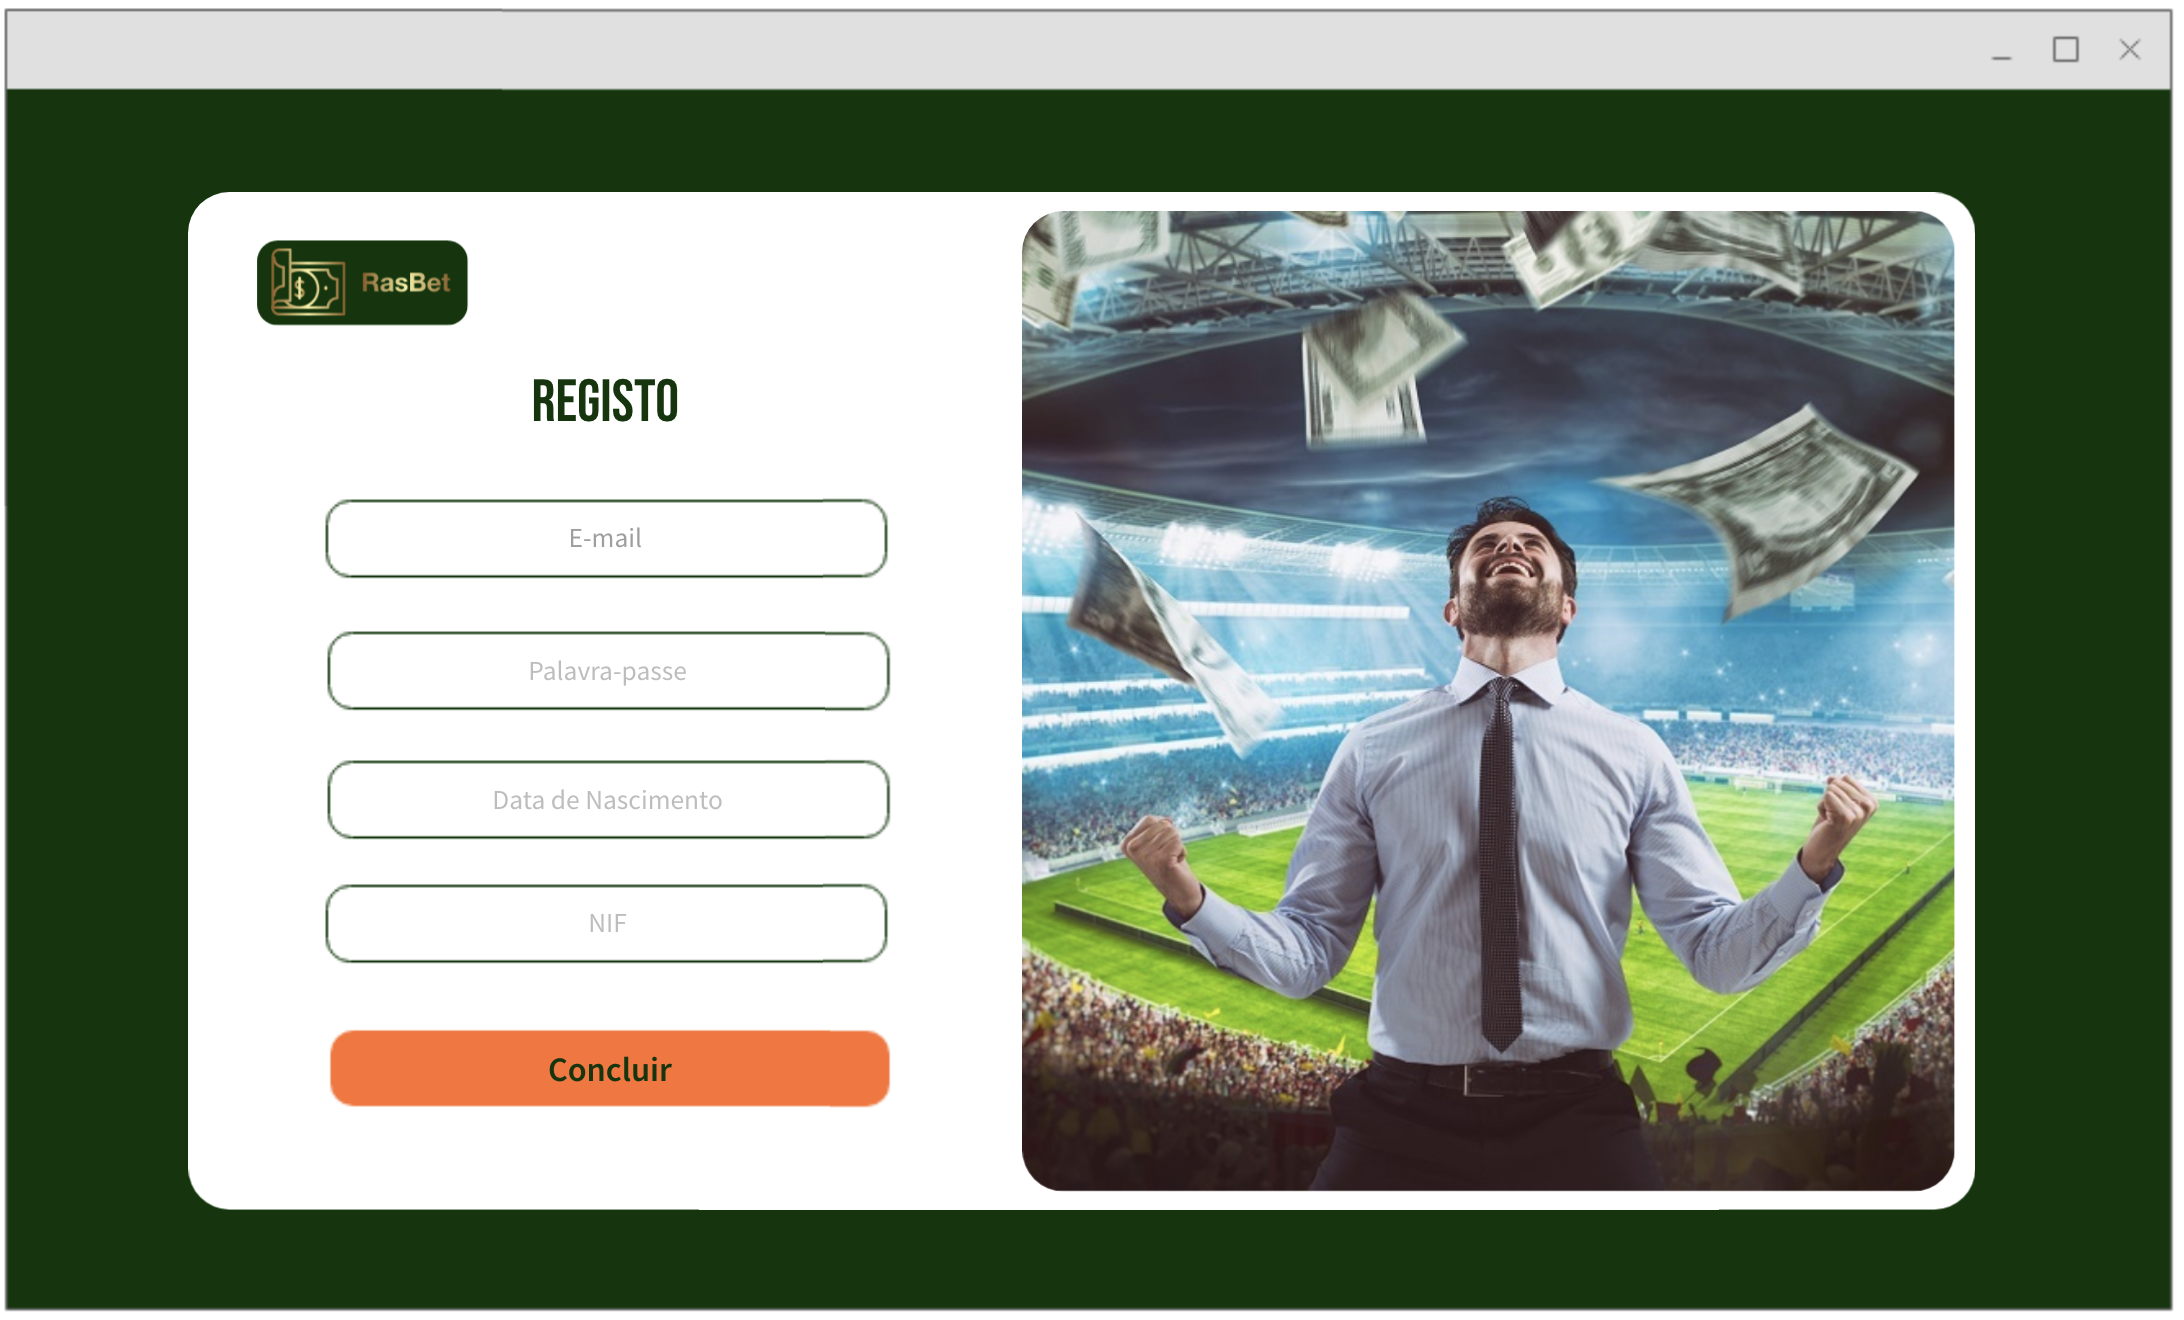
\includegraphics[width=0.9\textwidth]{imagens/ambitoProduto/Mockups/M_Registo.png}
\caption{Mockup de Registo}
\end{figure}

\subsection{Login Apostador/Especialista}
\begin{figure}[H]
\centering
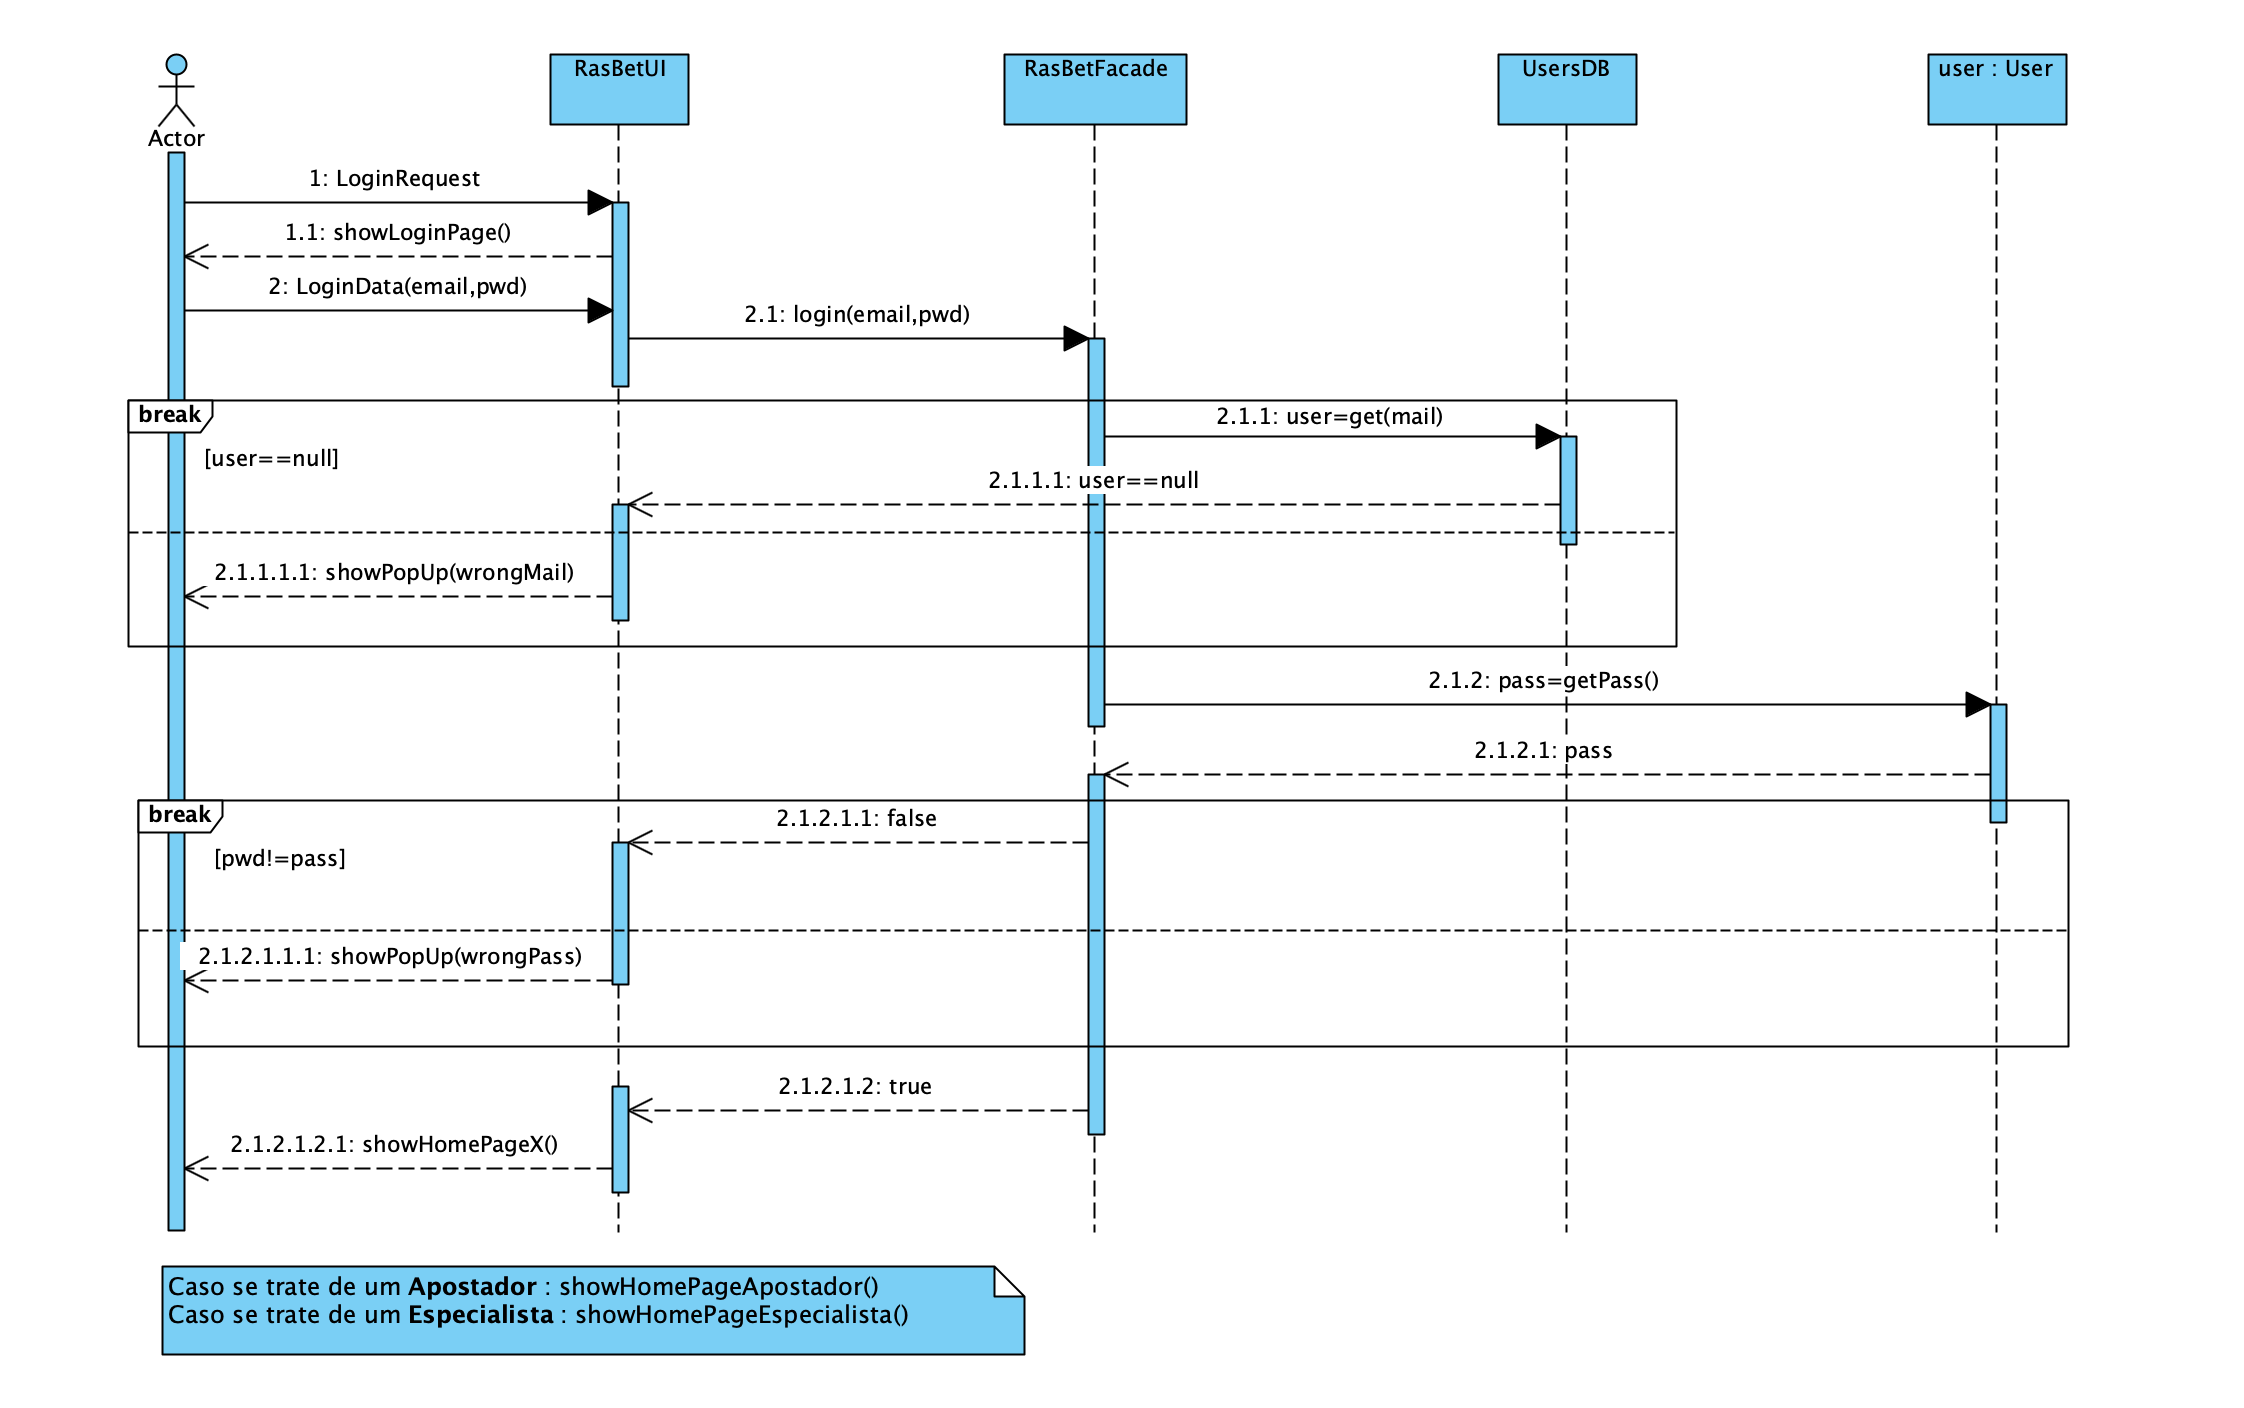
\includegraphics[width=1\textwidth]{imagens/ambitoProduto/SLogin.png}
\caption{Diagrama de Sequência de Login}
\end{figure}
\begin{figure}[H]
\centering
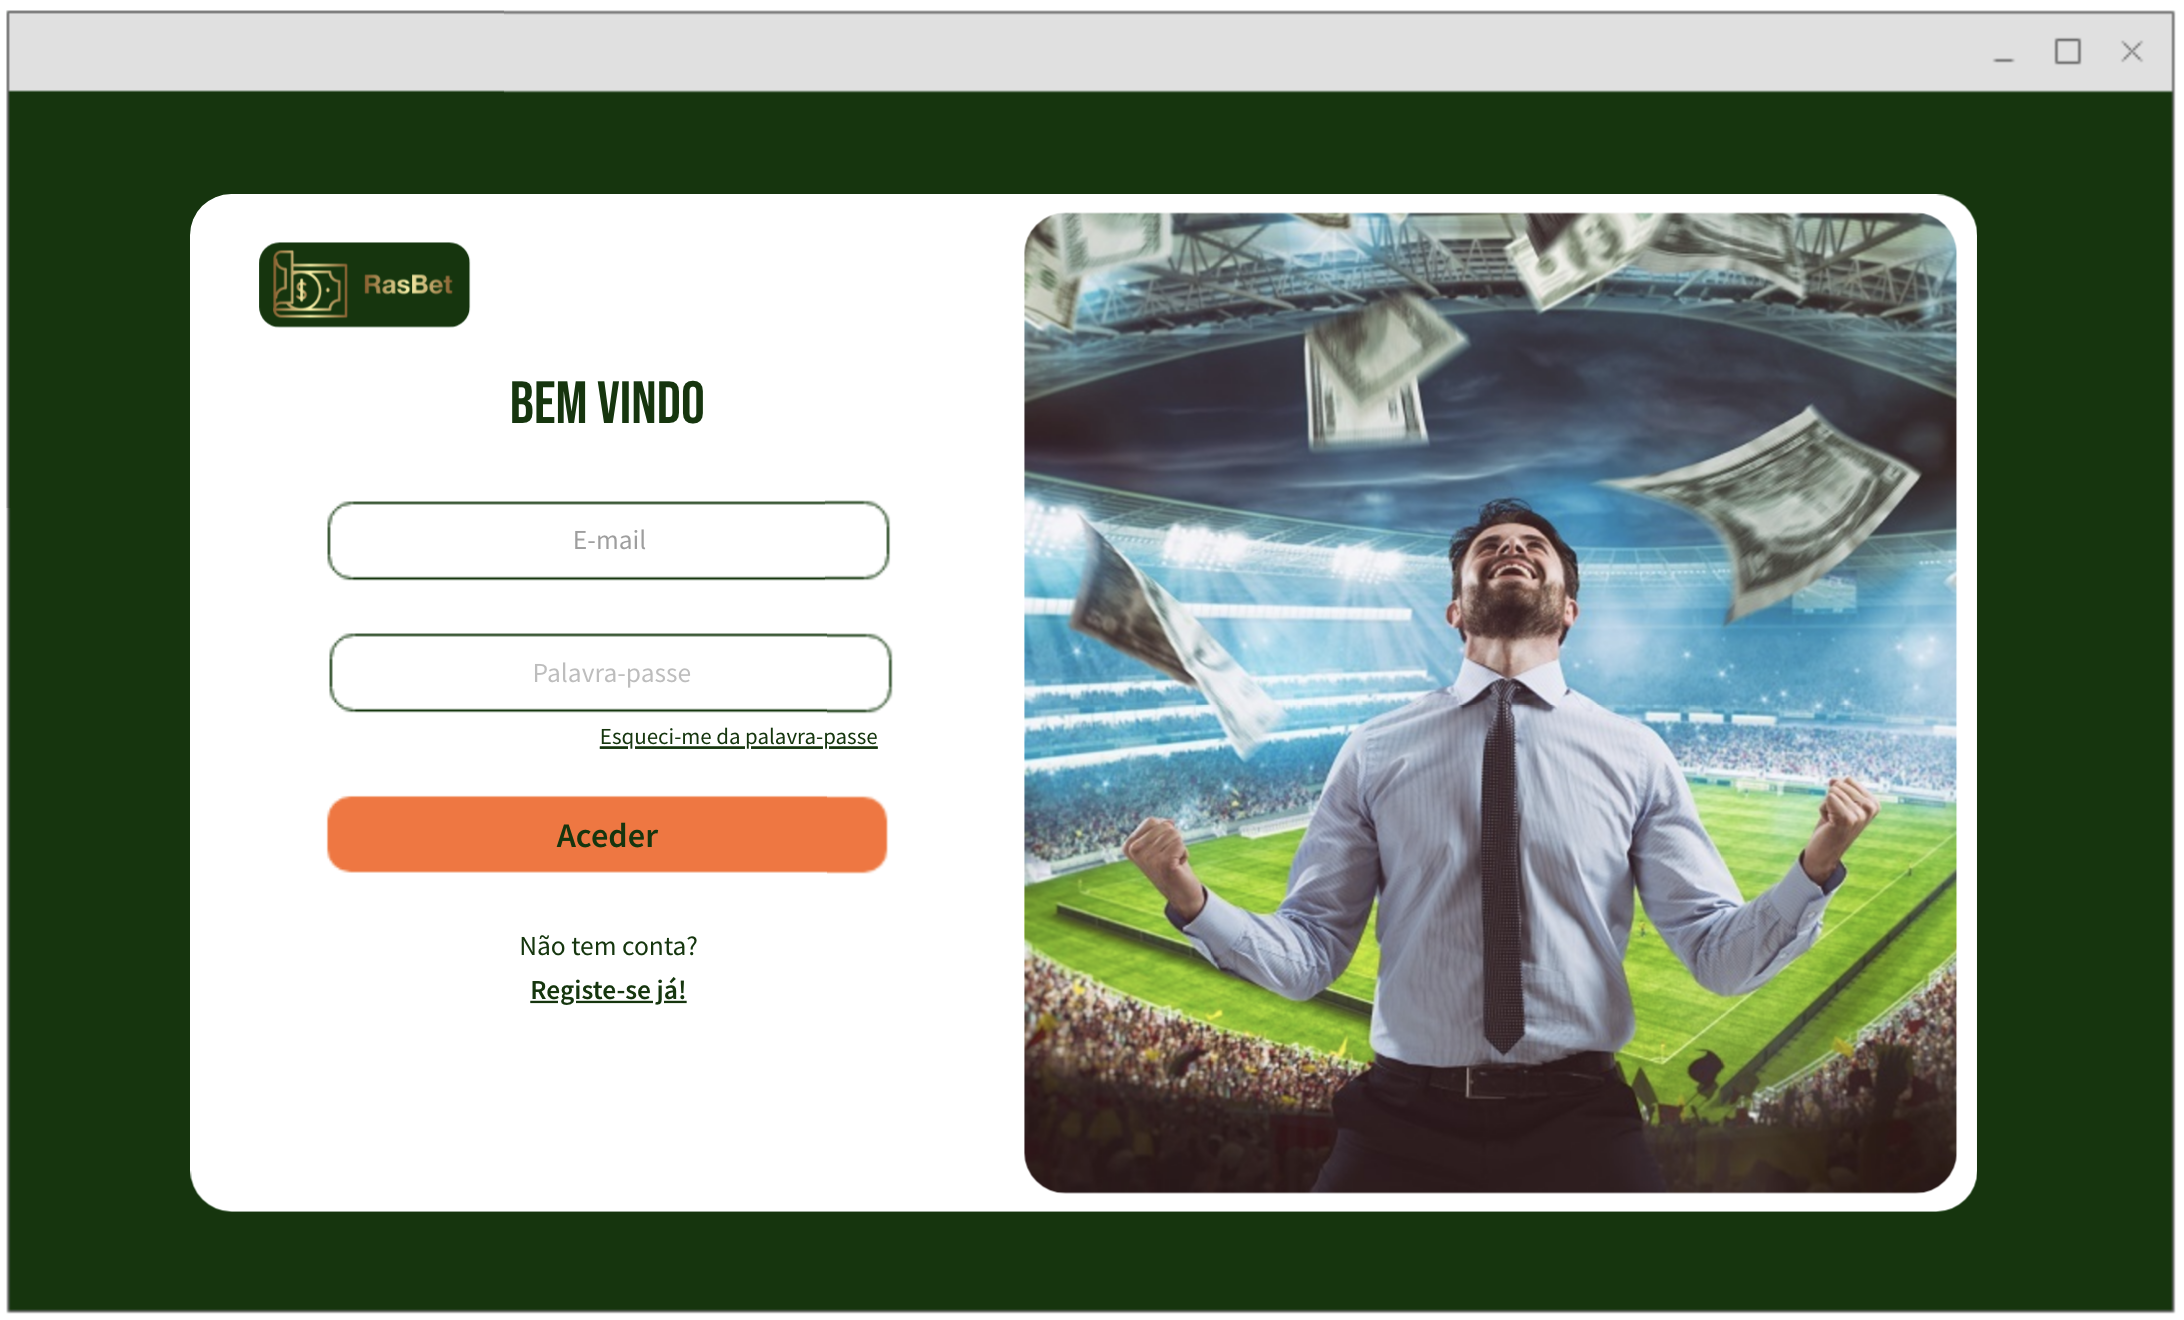
\includegraphics[width=1\textwidth]{imagens/ambitoProduto/Mockups/M_Login.png}
\caption{Mockup de Login}
\end{figure}

\subsection{Alterar informações de perfil}
\begin{figure}[H]
\centering
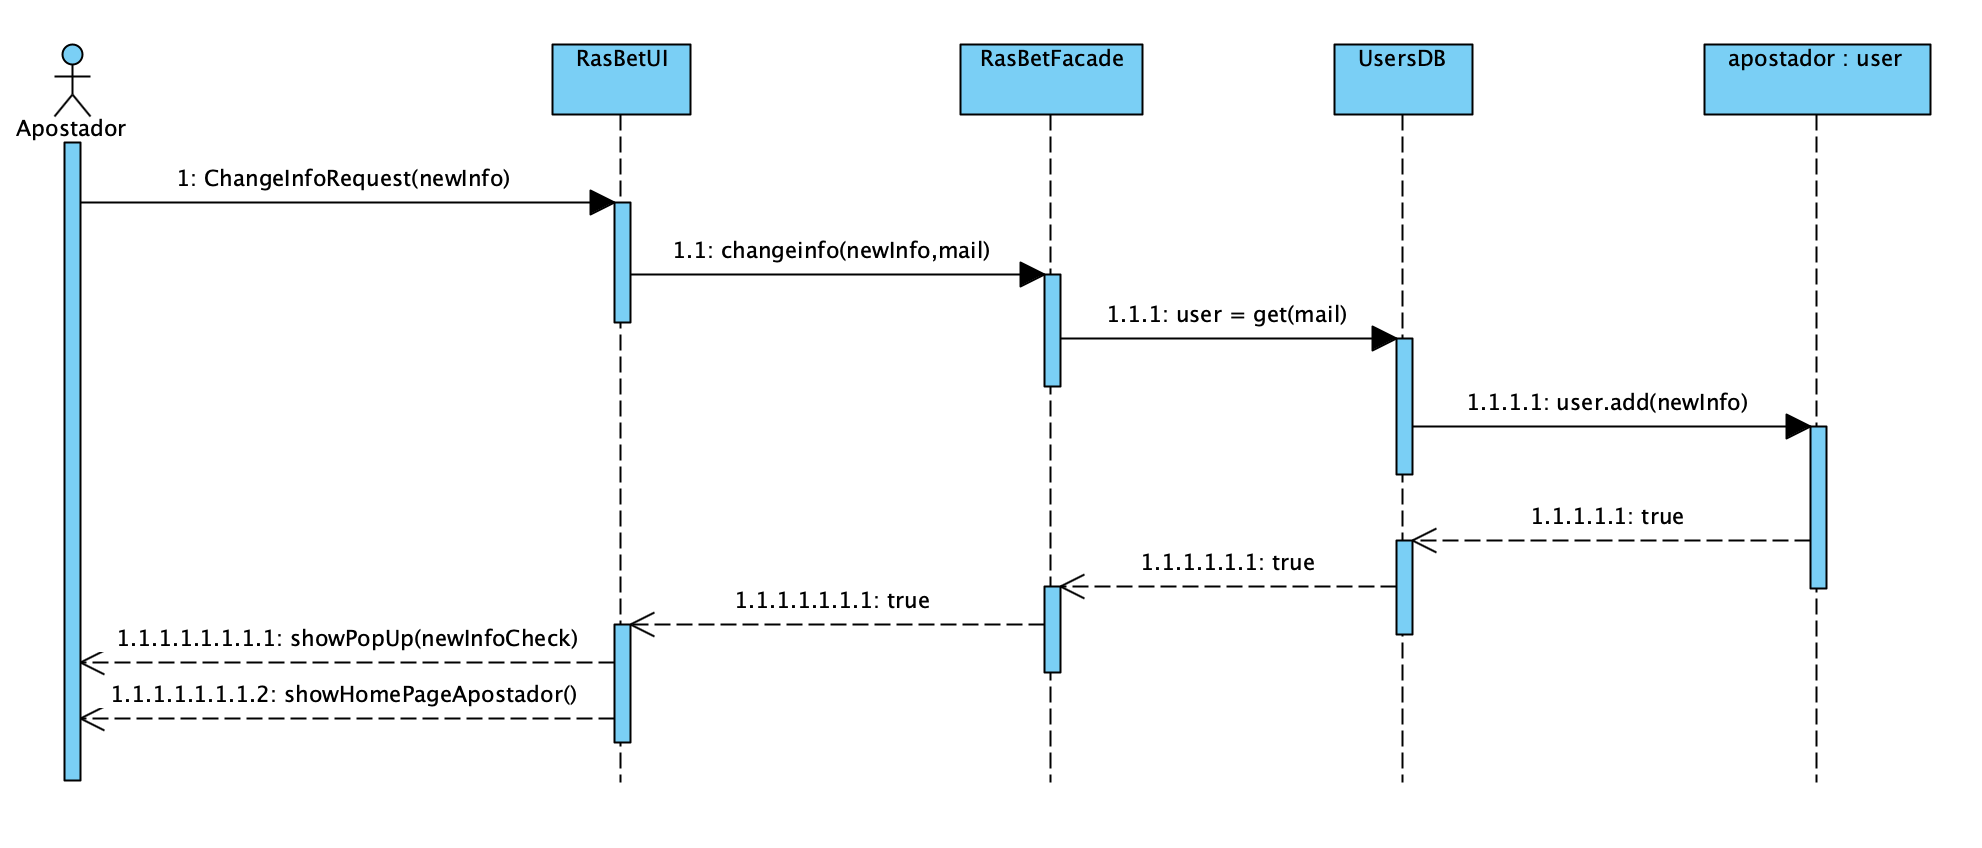
\includegraphics[width=1\textwidth]{imagens/ambitoProduto/SalterarInfo.png}
\caption{Diagrama de Sequência de alterar informações de perfil}
\end{figure}
\begin{figure}[H]
\centering
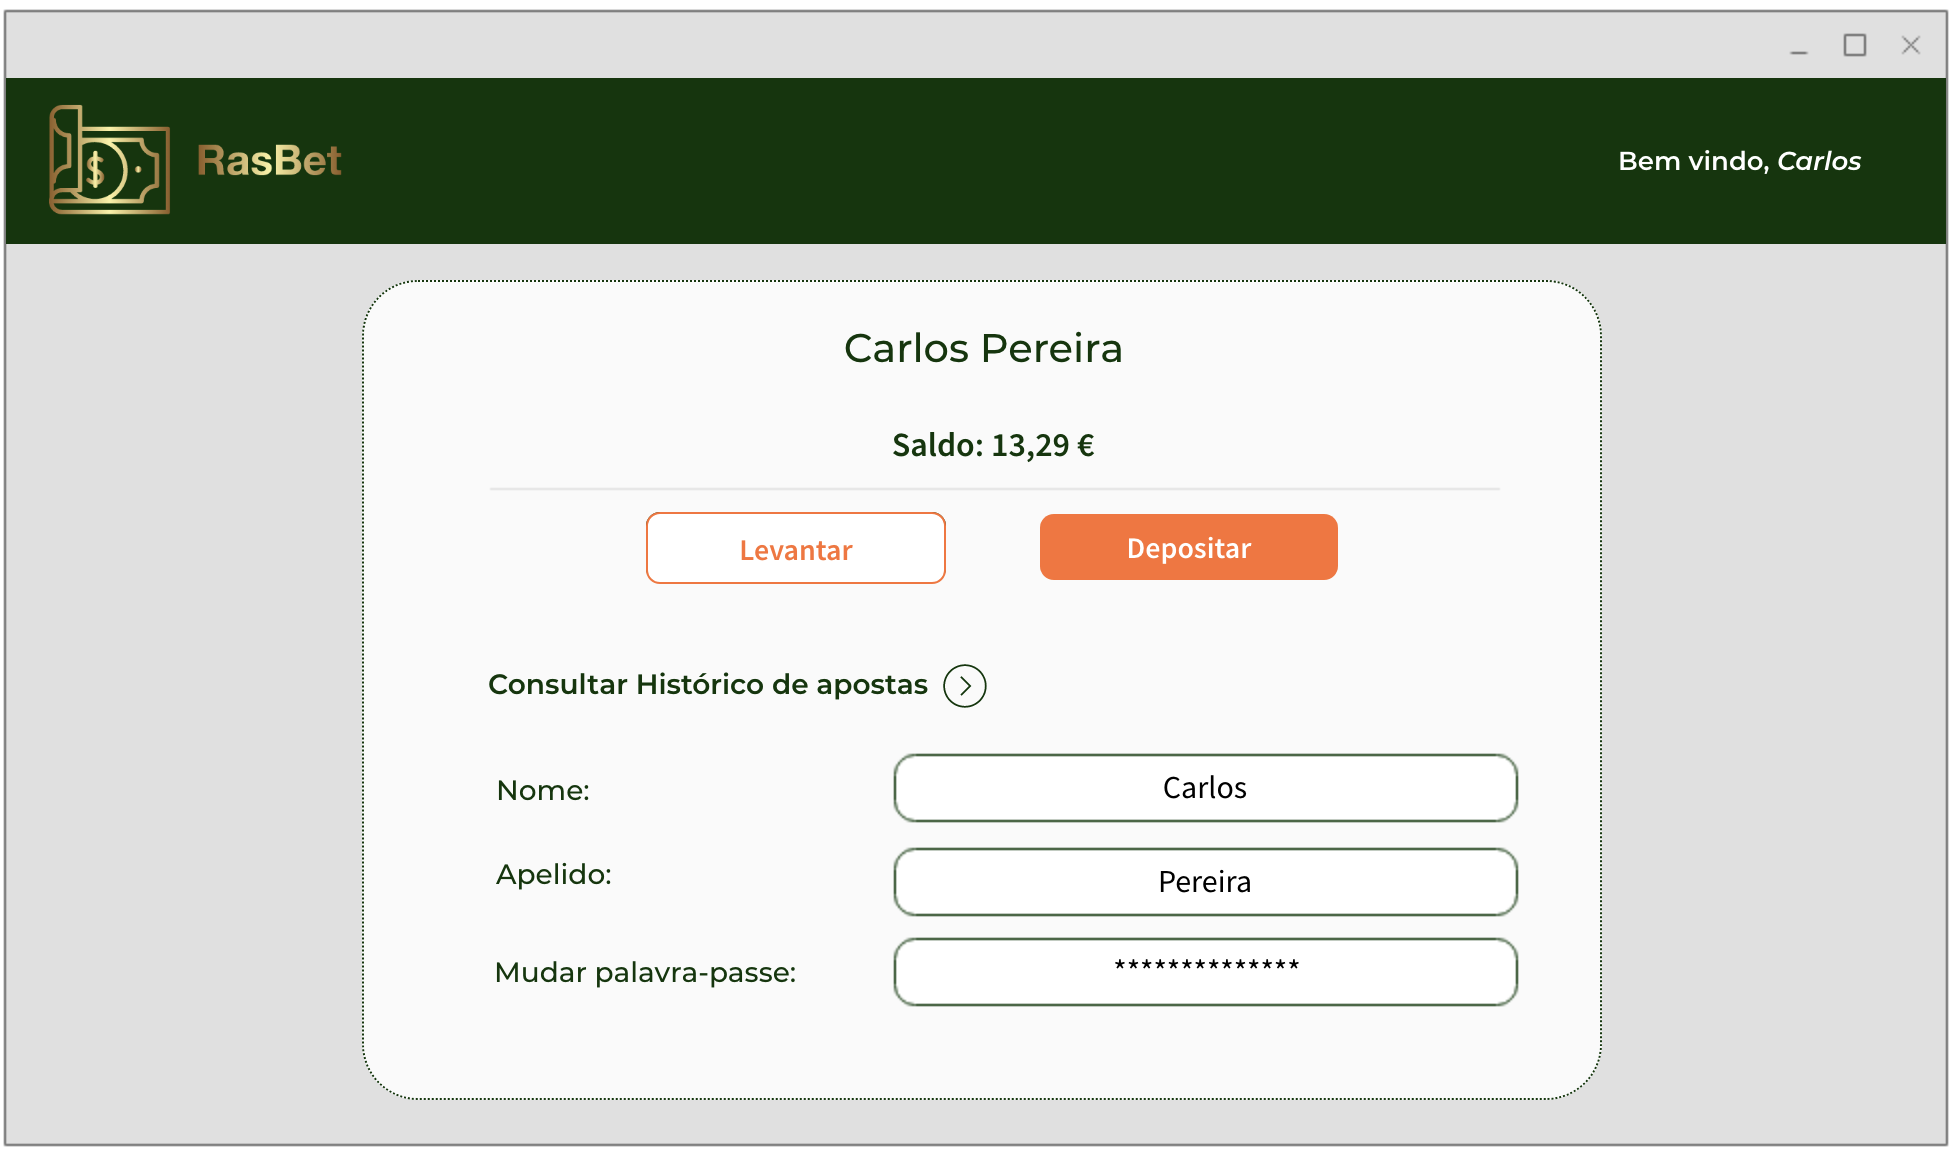
\includegraphics[width=1\textwidth]{imagens/ambitoProduto/Mockups/M_Configuracoes.png}
\caption{Mockup de Alterar informações de perfil}
\end{figure}

\subsection{Consultar jogos}
\begin{figure}[H]
\centering
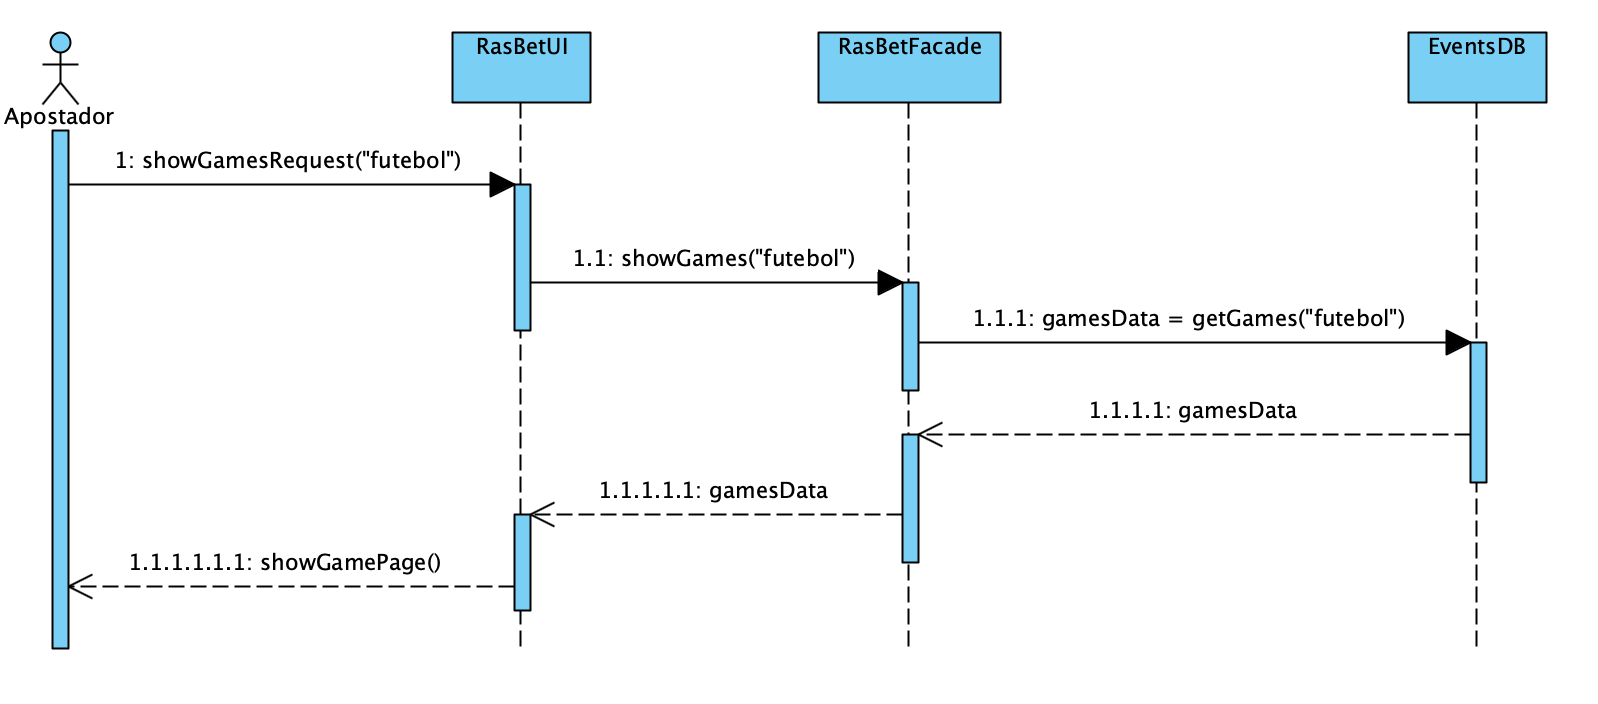
\includegraphics[width=1\textwidth]{imagens/ambitoProduto/SConsultaJogo.png}
\caption{Diagrama de Sequência de Consultar jogos}
\end{figure}
\begin{figure}[H]
\centering
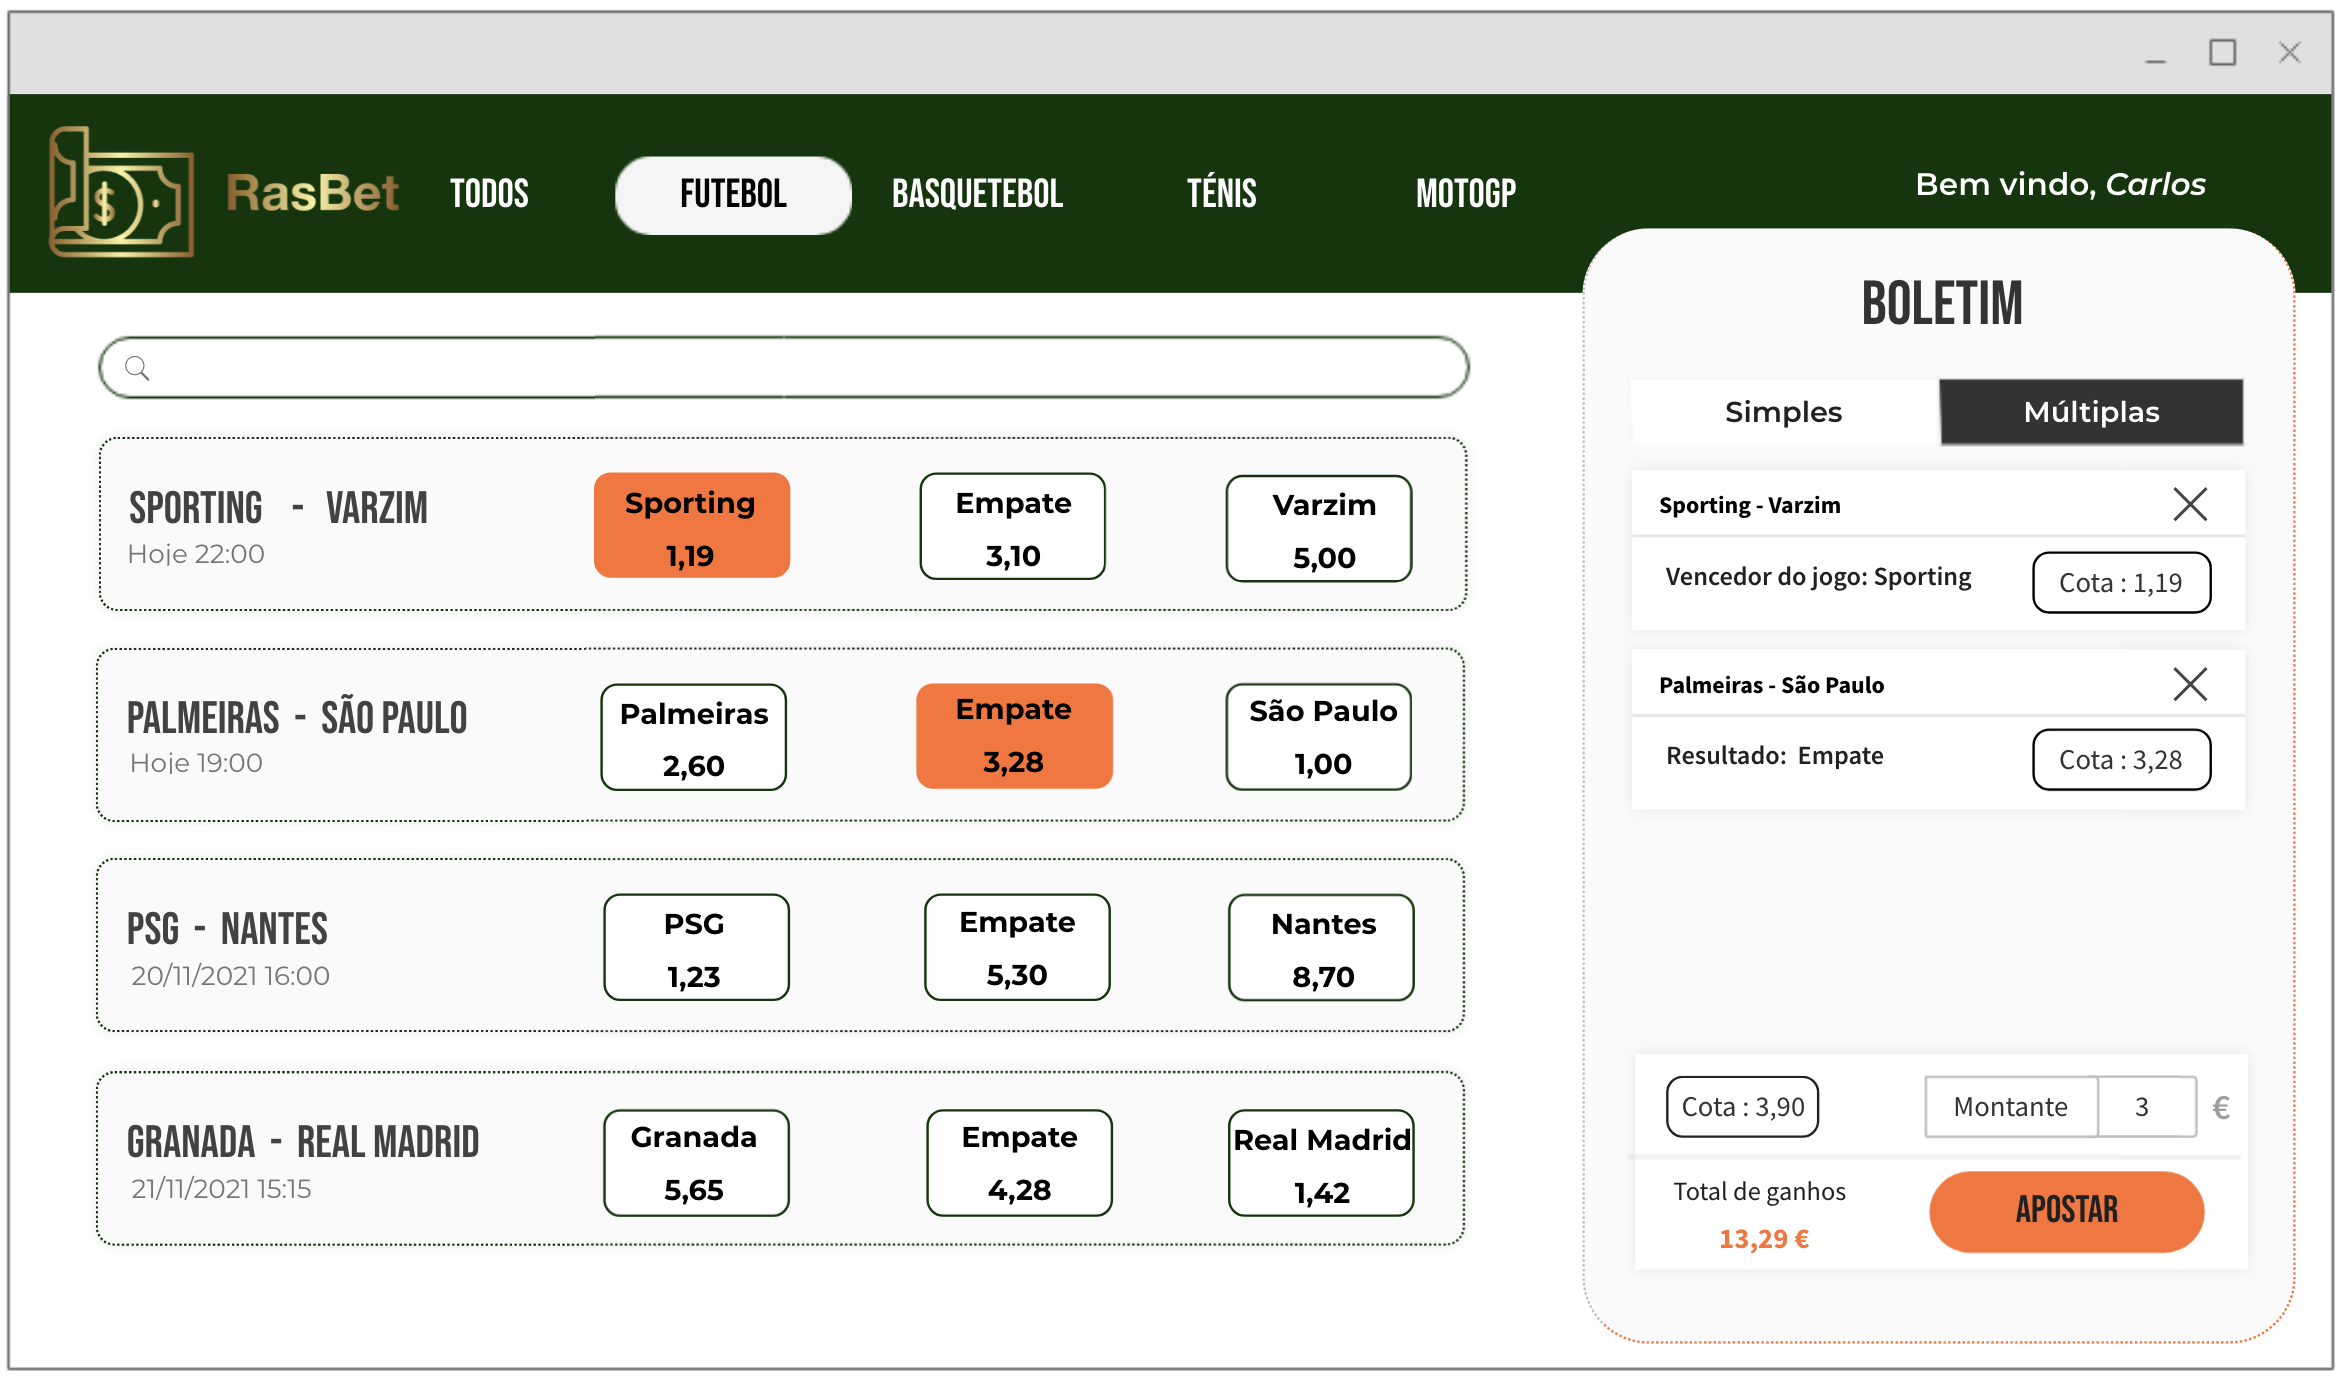
\includegraphics[width=1\textwidth]{imagens/ambitoProduto/Mockups/M_consultarJogos.png}
\caption{Mockup de Consultar jogos}
\end{figure}

\subsection{Fazer Aposta}
\begin{figure}[H]
\centering
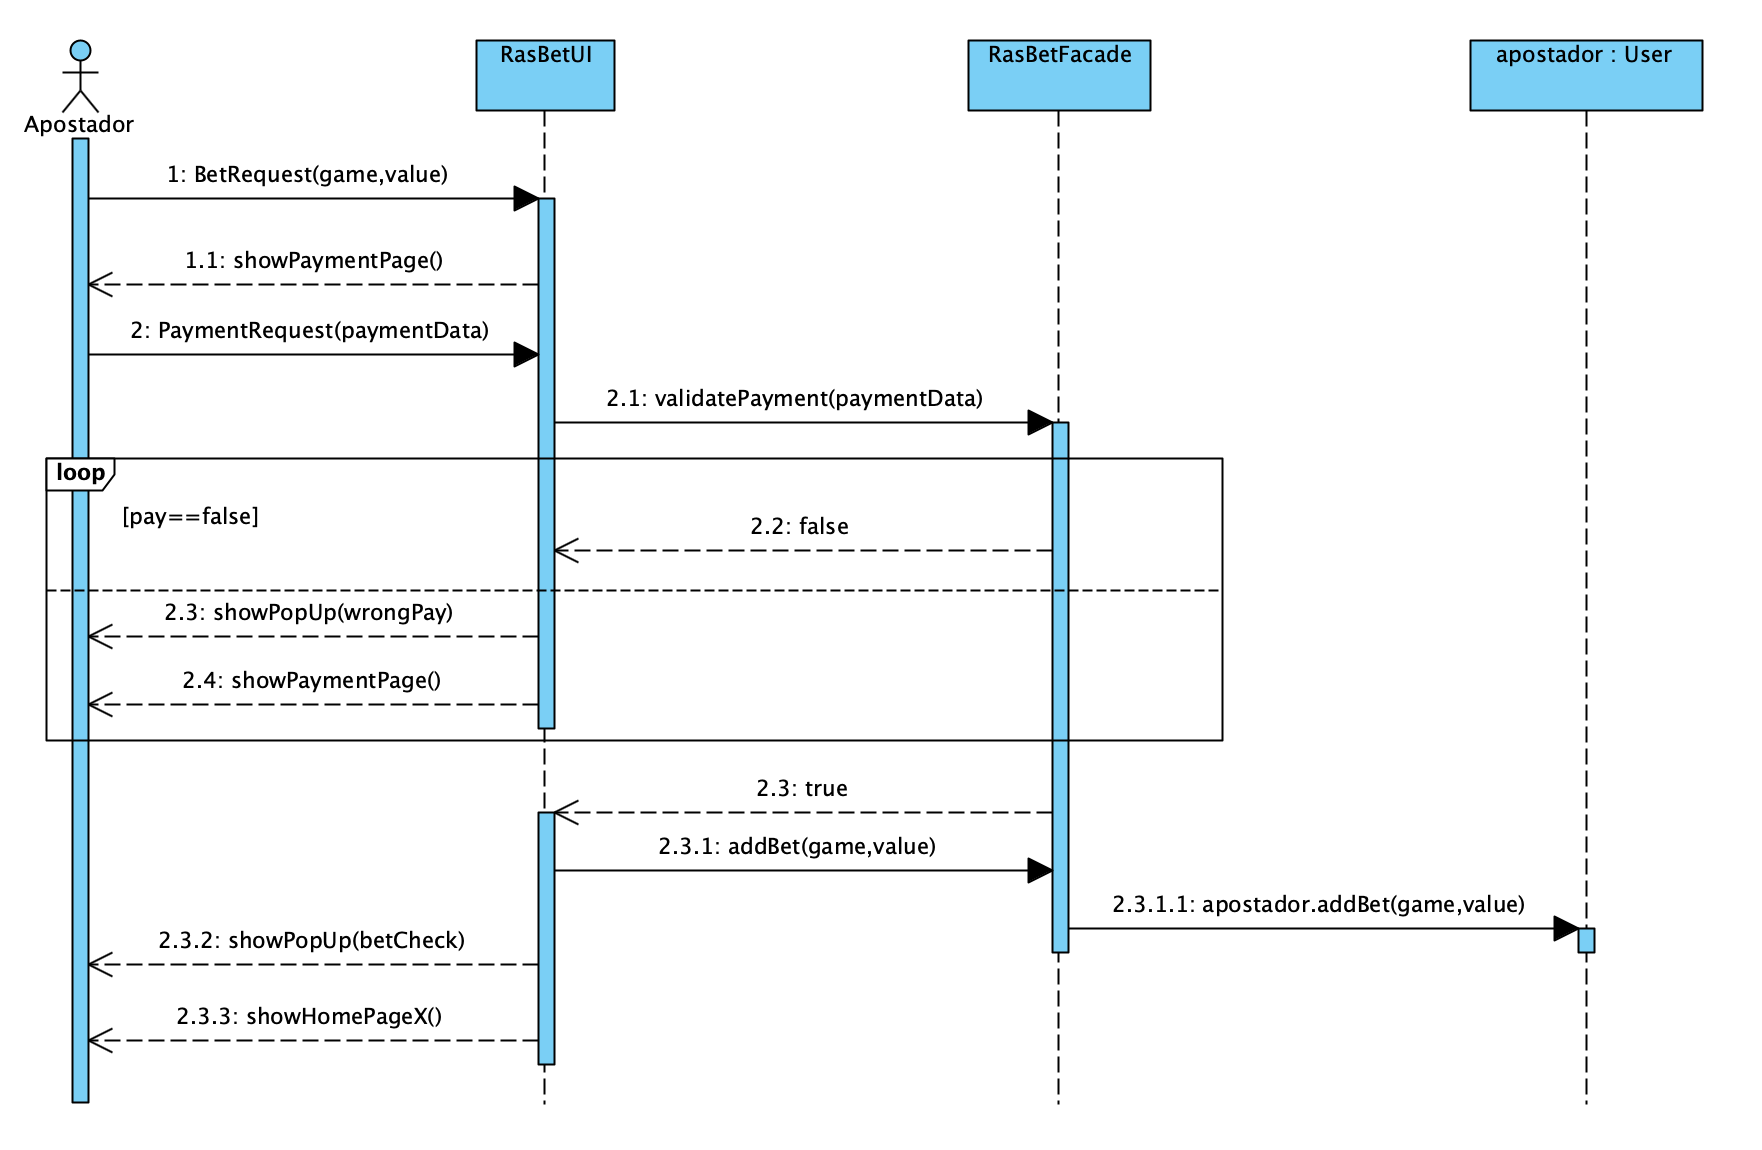
\includegraphics[width=1\textwidth]{imagens/ambitoProduto/SFazerAposta.png}
\caption{Diagrama de Sequência de Consultar jogos}
\end{figure}

\begin{figure}[H]
\centering
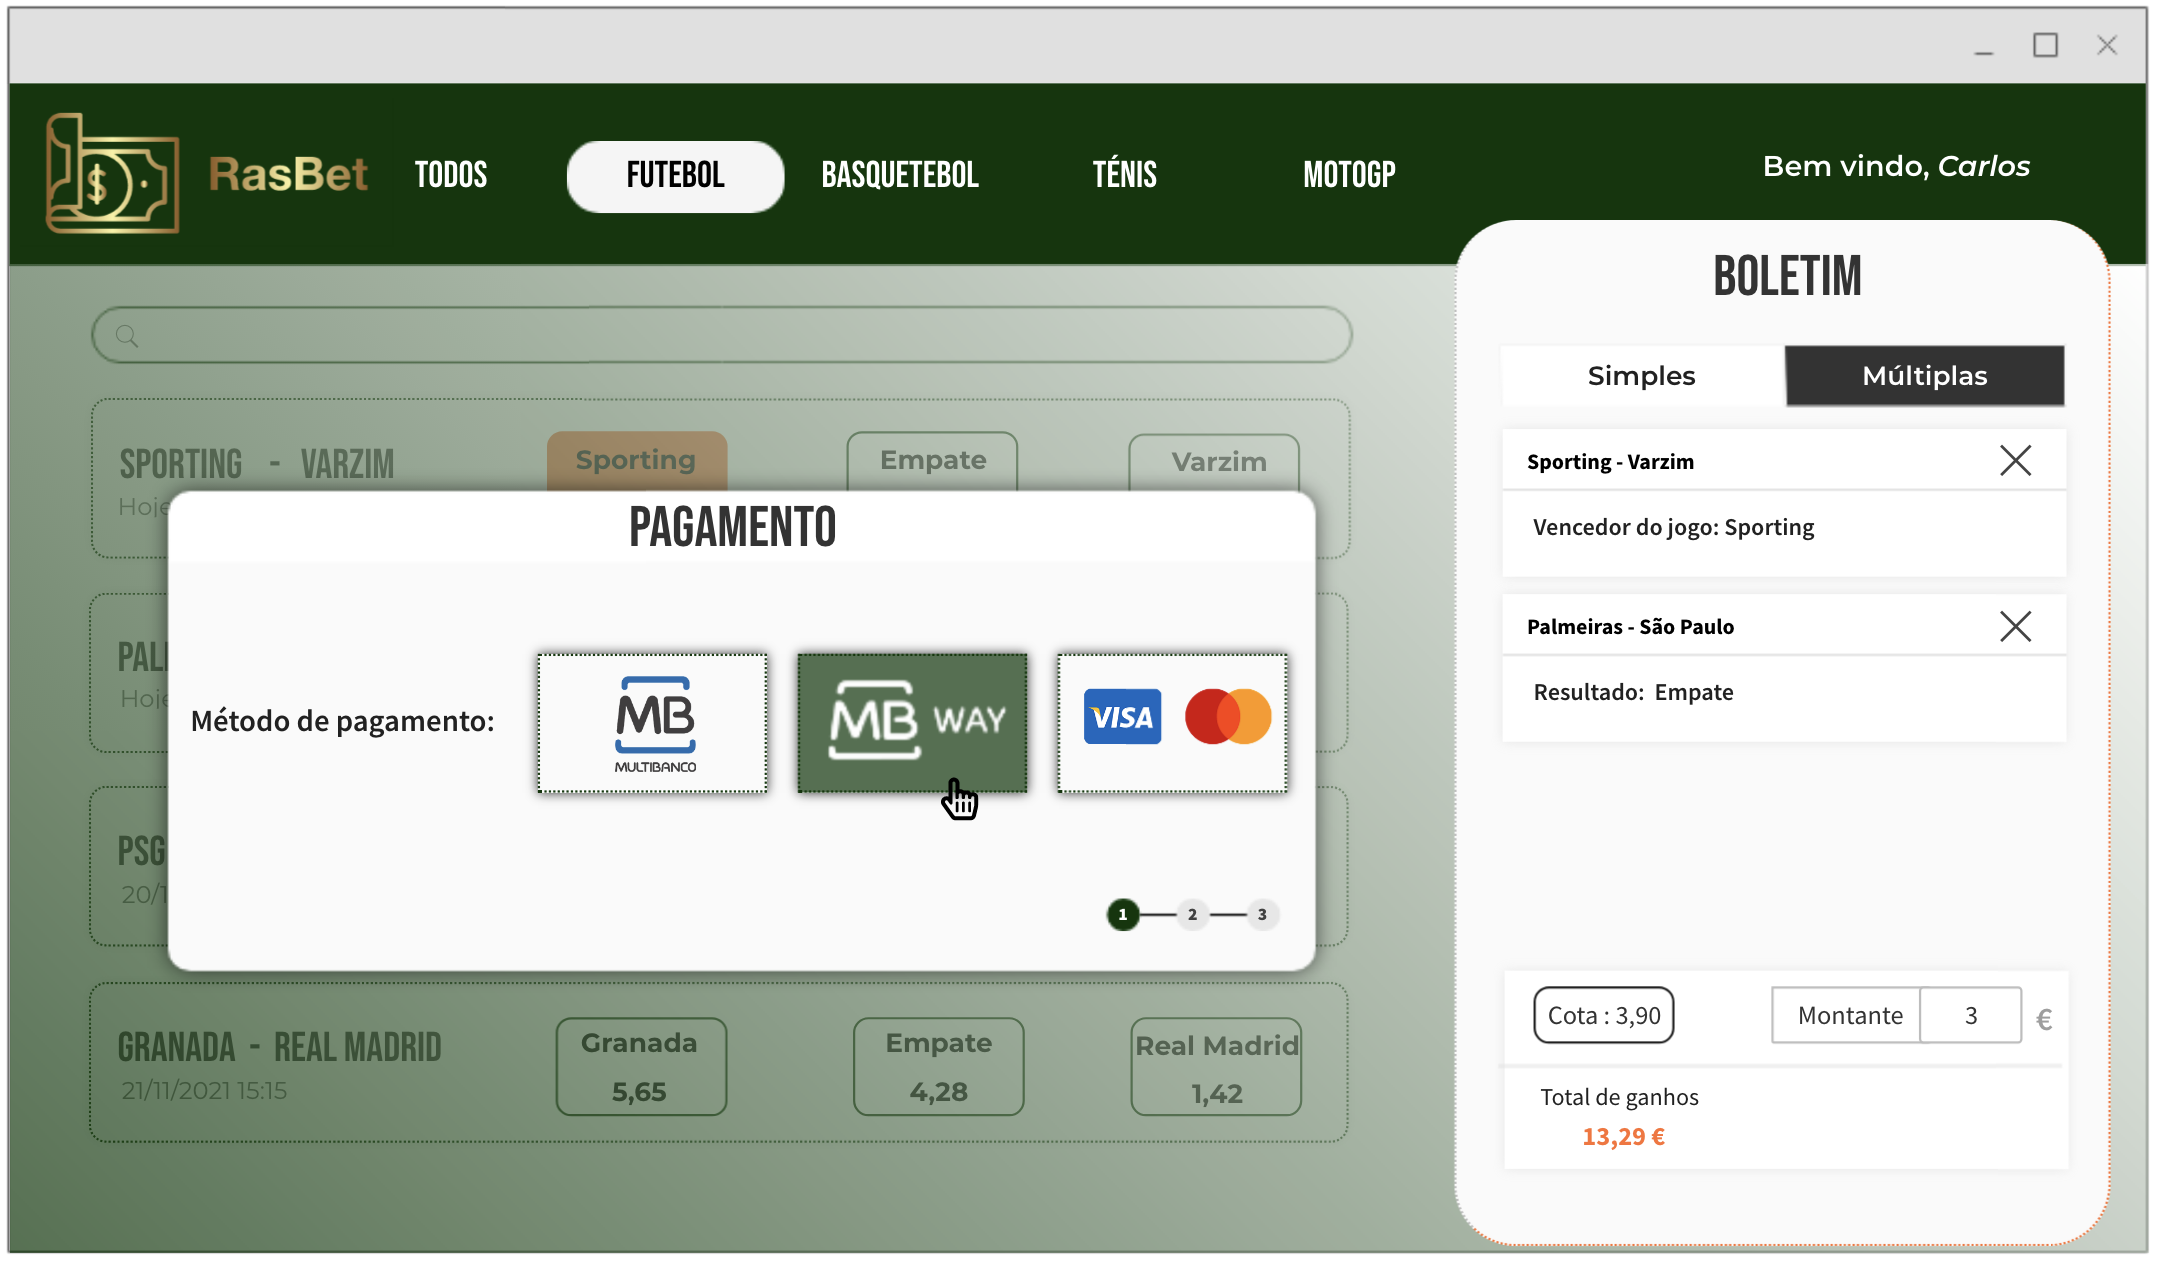
\includegraphics[width=1\textwidth]{imagens/ambitoProduto/Mockups/M_Apostar1.png}
\caption{Mockup de Fazer Aposta 1}
\end{figure}
\begin{figure}[H]
\centering
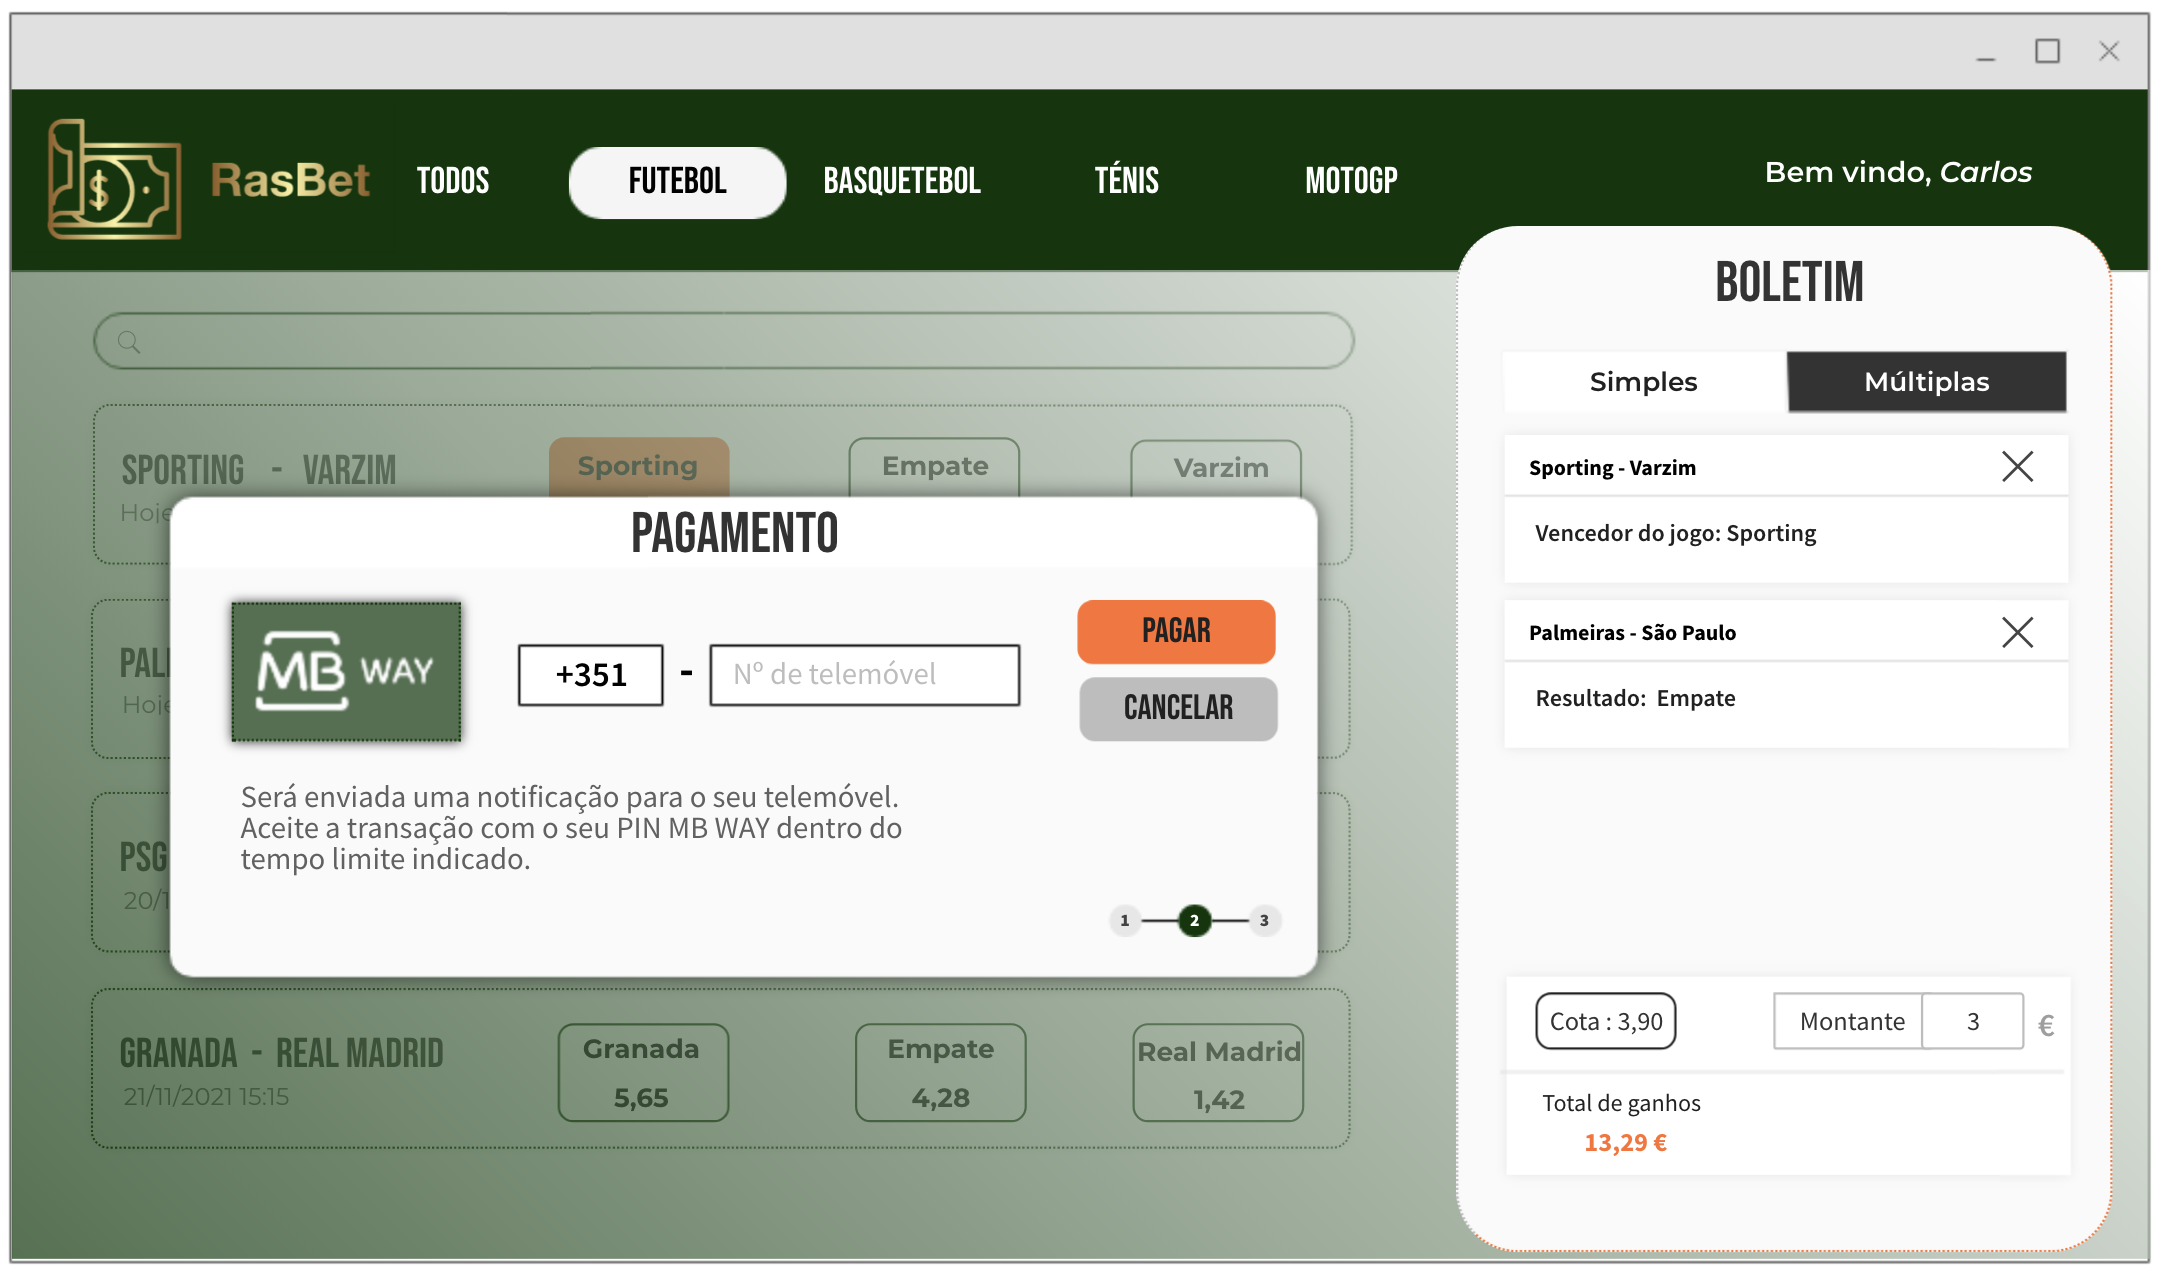
\includegraphics[width=1\textwidth]{imagens/ambitoProduto/Mockups/M_Apostar2.png}
\caption{Mockup de Fazer Aposta 2}
\end{figure}
\begin{figure}[H]
\centering
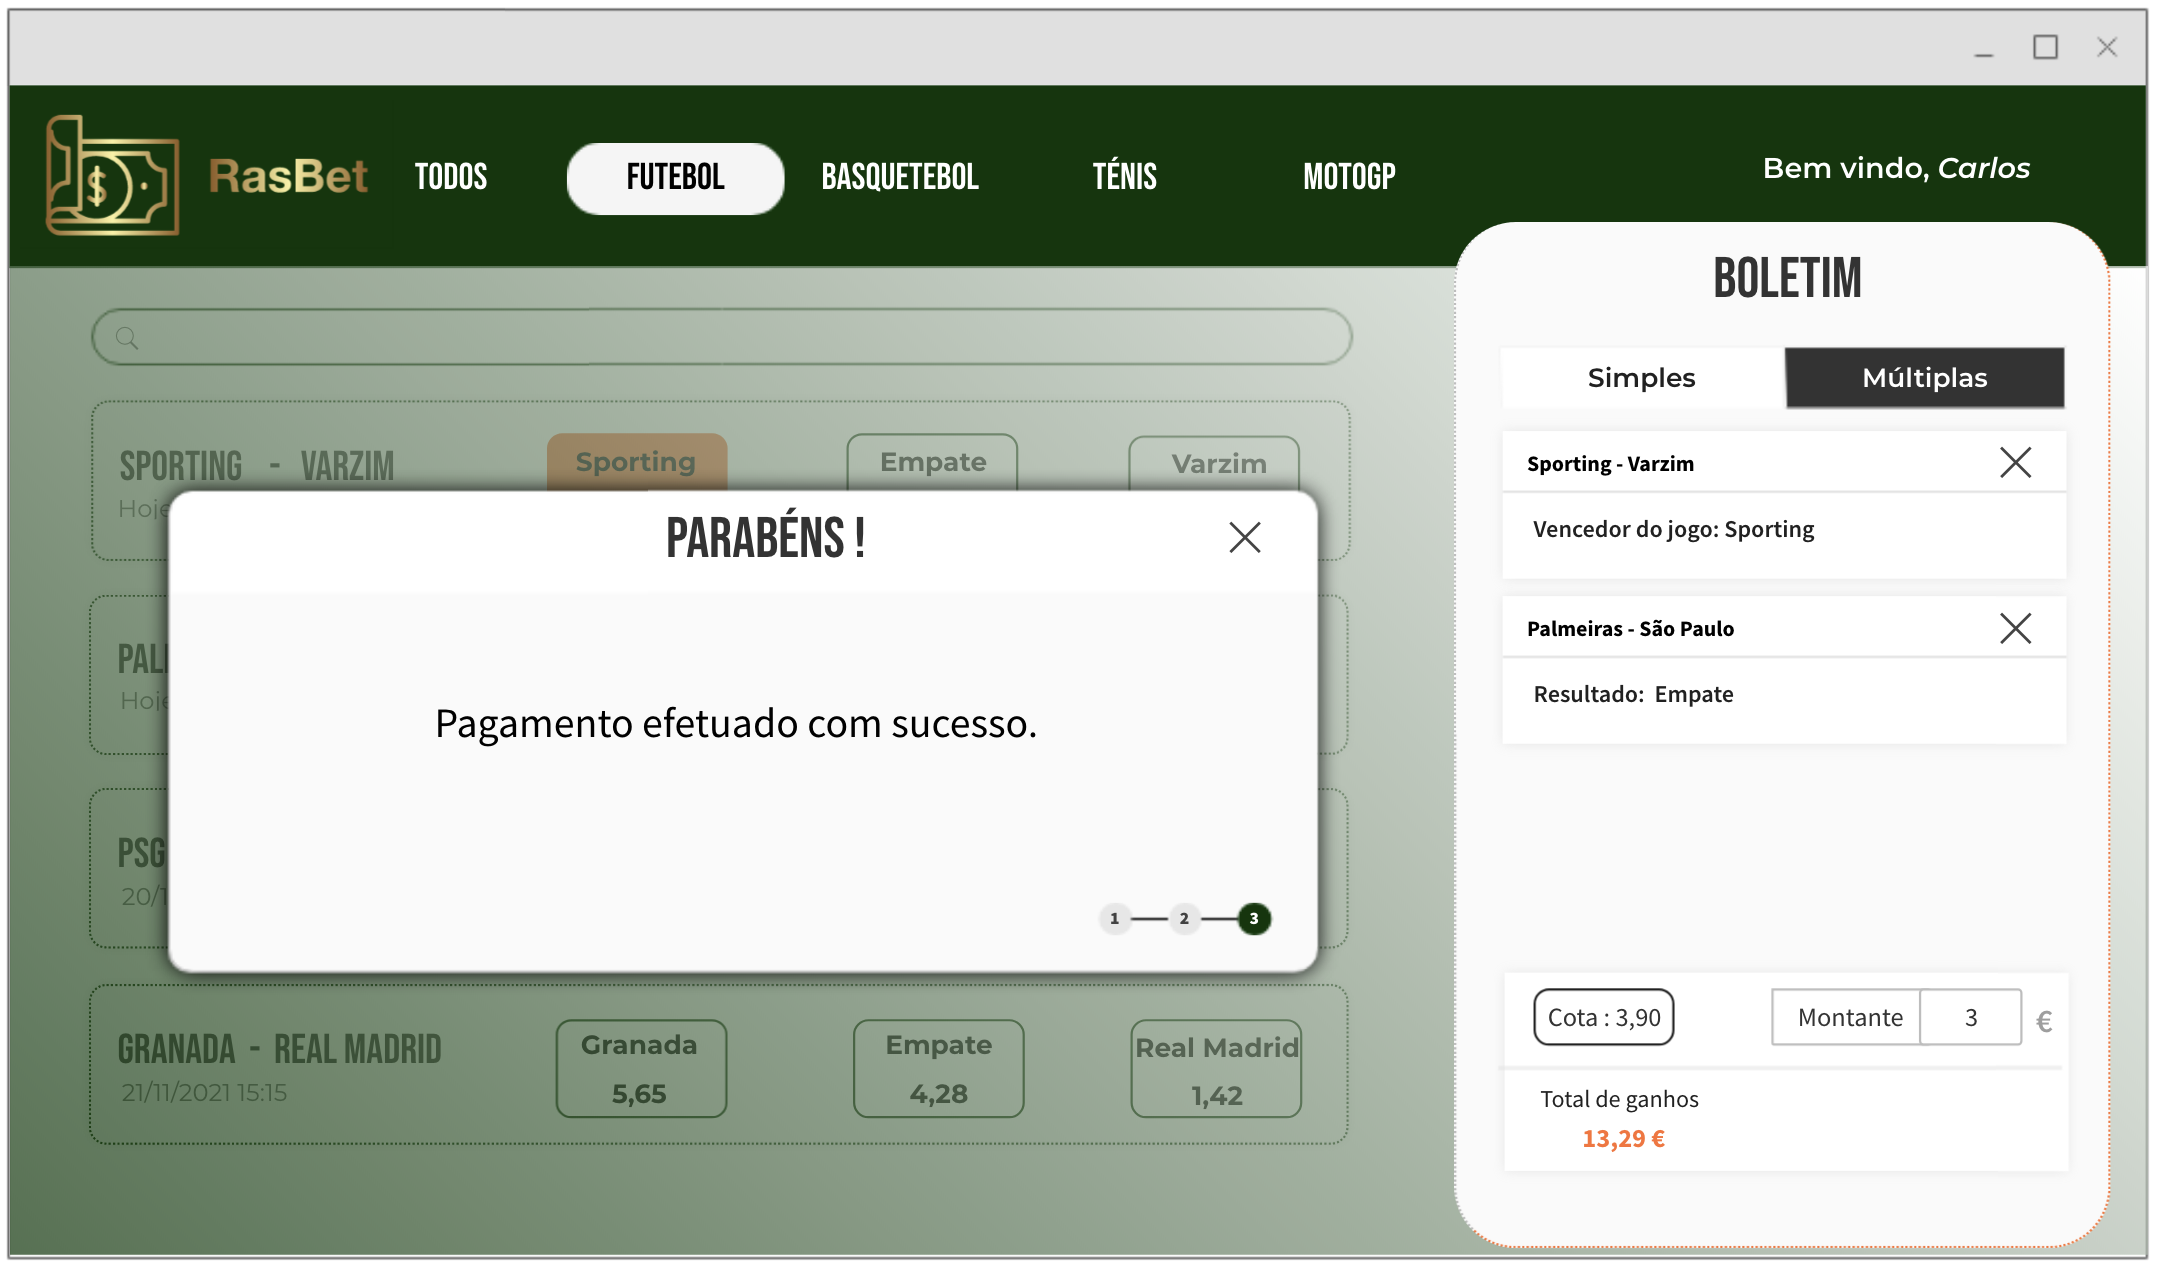
\includegraphics[width=1\textwidth]{imagens/ambitoProduto/Mockups/M_Apostar3.png}
\caption{Mockup de Fazer Aposta 3}
\end{figure}

\subsection{Consultar histórico de Apostas}
\begin{figure}[H]
\centering
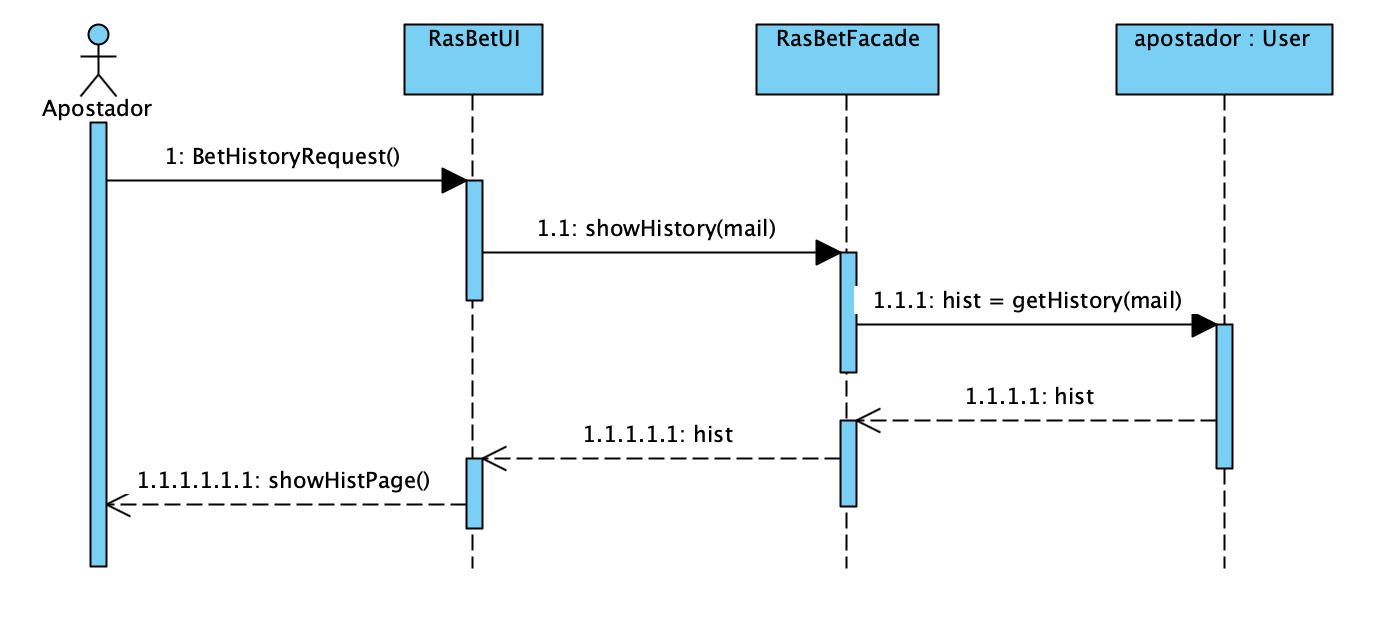
\includegraphics[width=1\textwidth]{imagens/ambitoProduto/SconsultaA.png}
\caption{Diagrama de Sequência de Consultar histórico de Apostas}
\end{figure}
\begin{figure}[H]
\centering
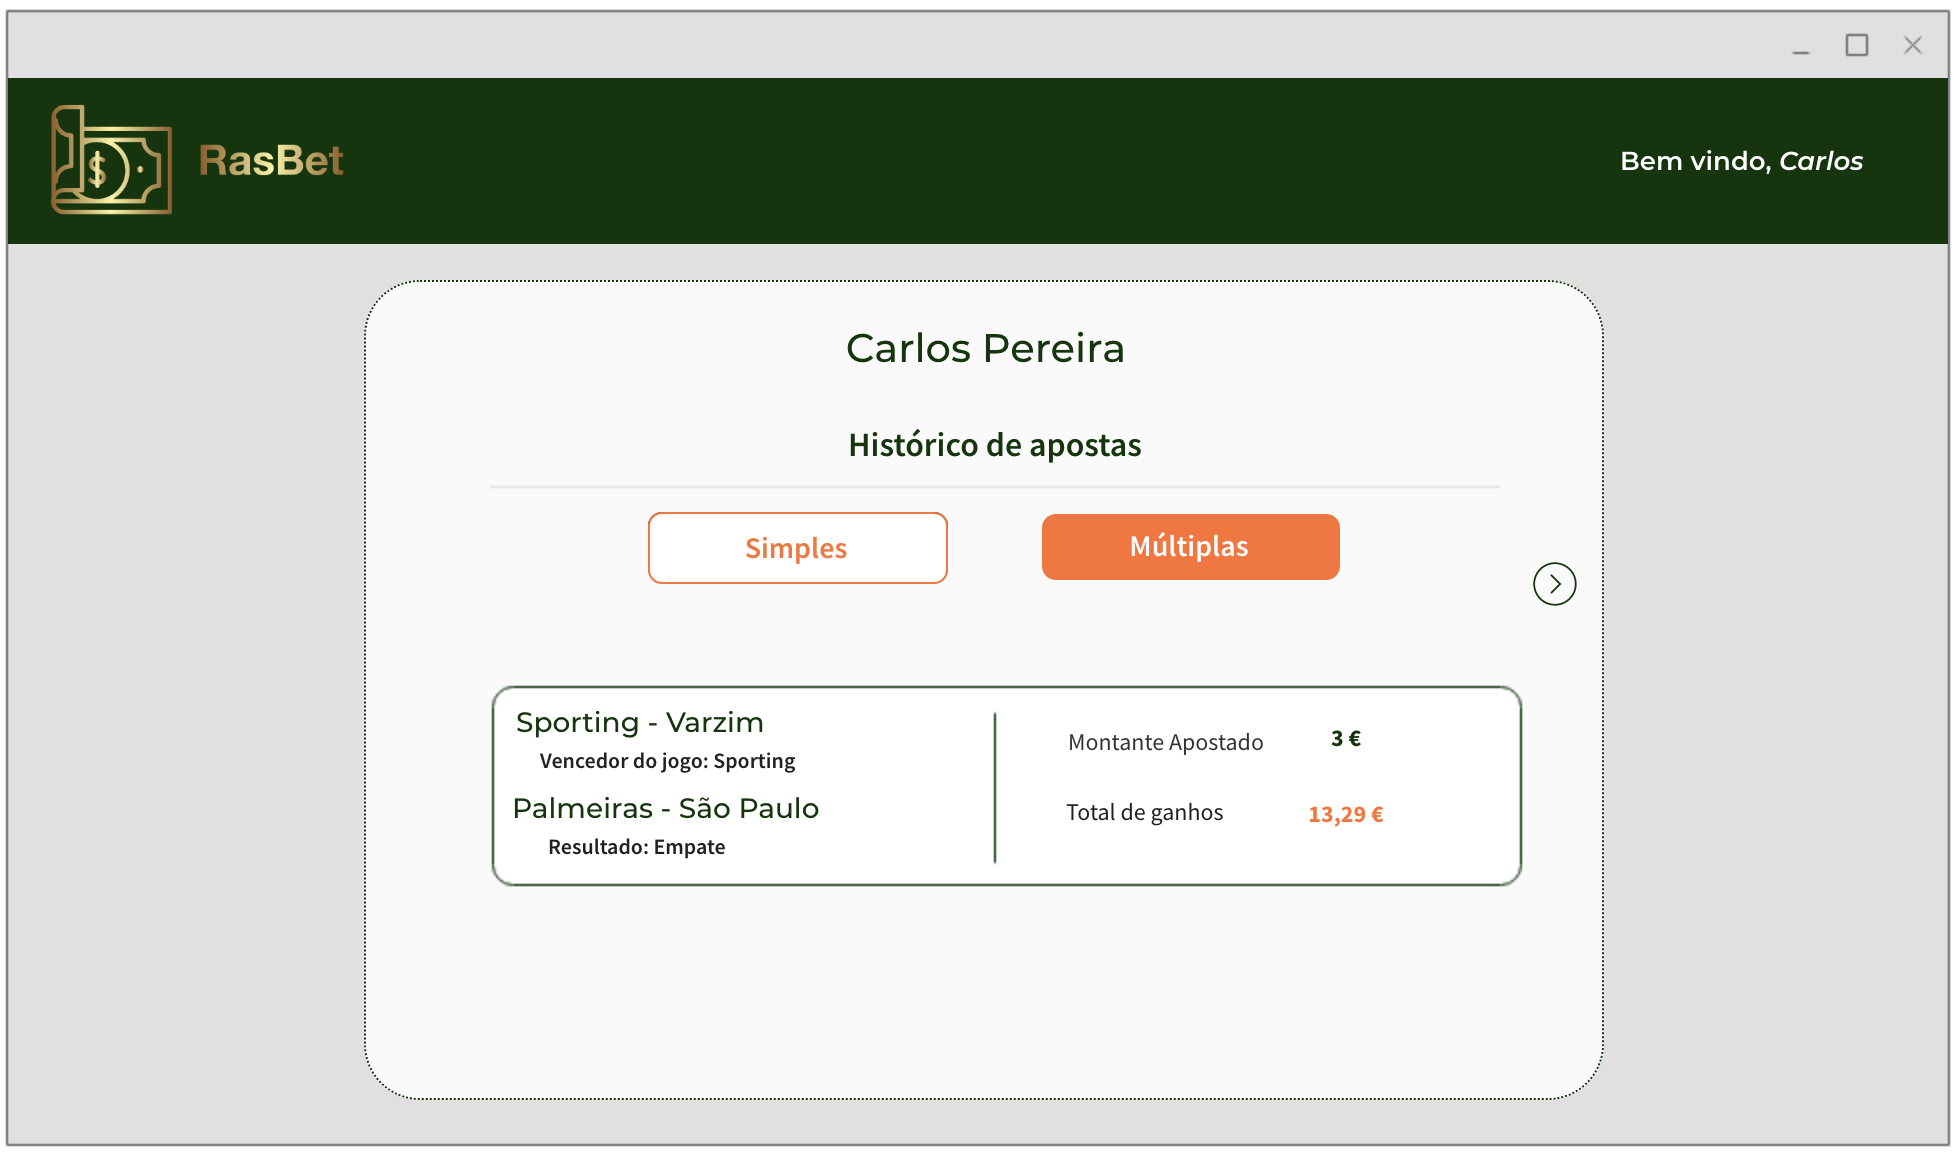
\includegraphics[width=1\textwidth]{imagens/ambitoProduto/Mockups/M_HistoricoApostas.png}
\caption{Mockup de Consultar histórico de Apostas}
\end{figure}

\subsection{Consultar histórico de transações}
\begin{figure}[H]
\centering
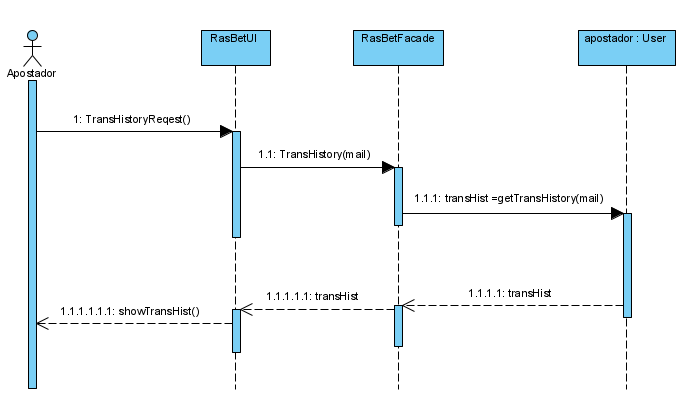
\includegraphics[width=1\textwidth]{imagens/ambitoProduto/STransHistory.png}
\caption{Diagrama de Sequência de Consultar histórico de transações}
\end{figure}
\begin{figure}[H]
\centering
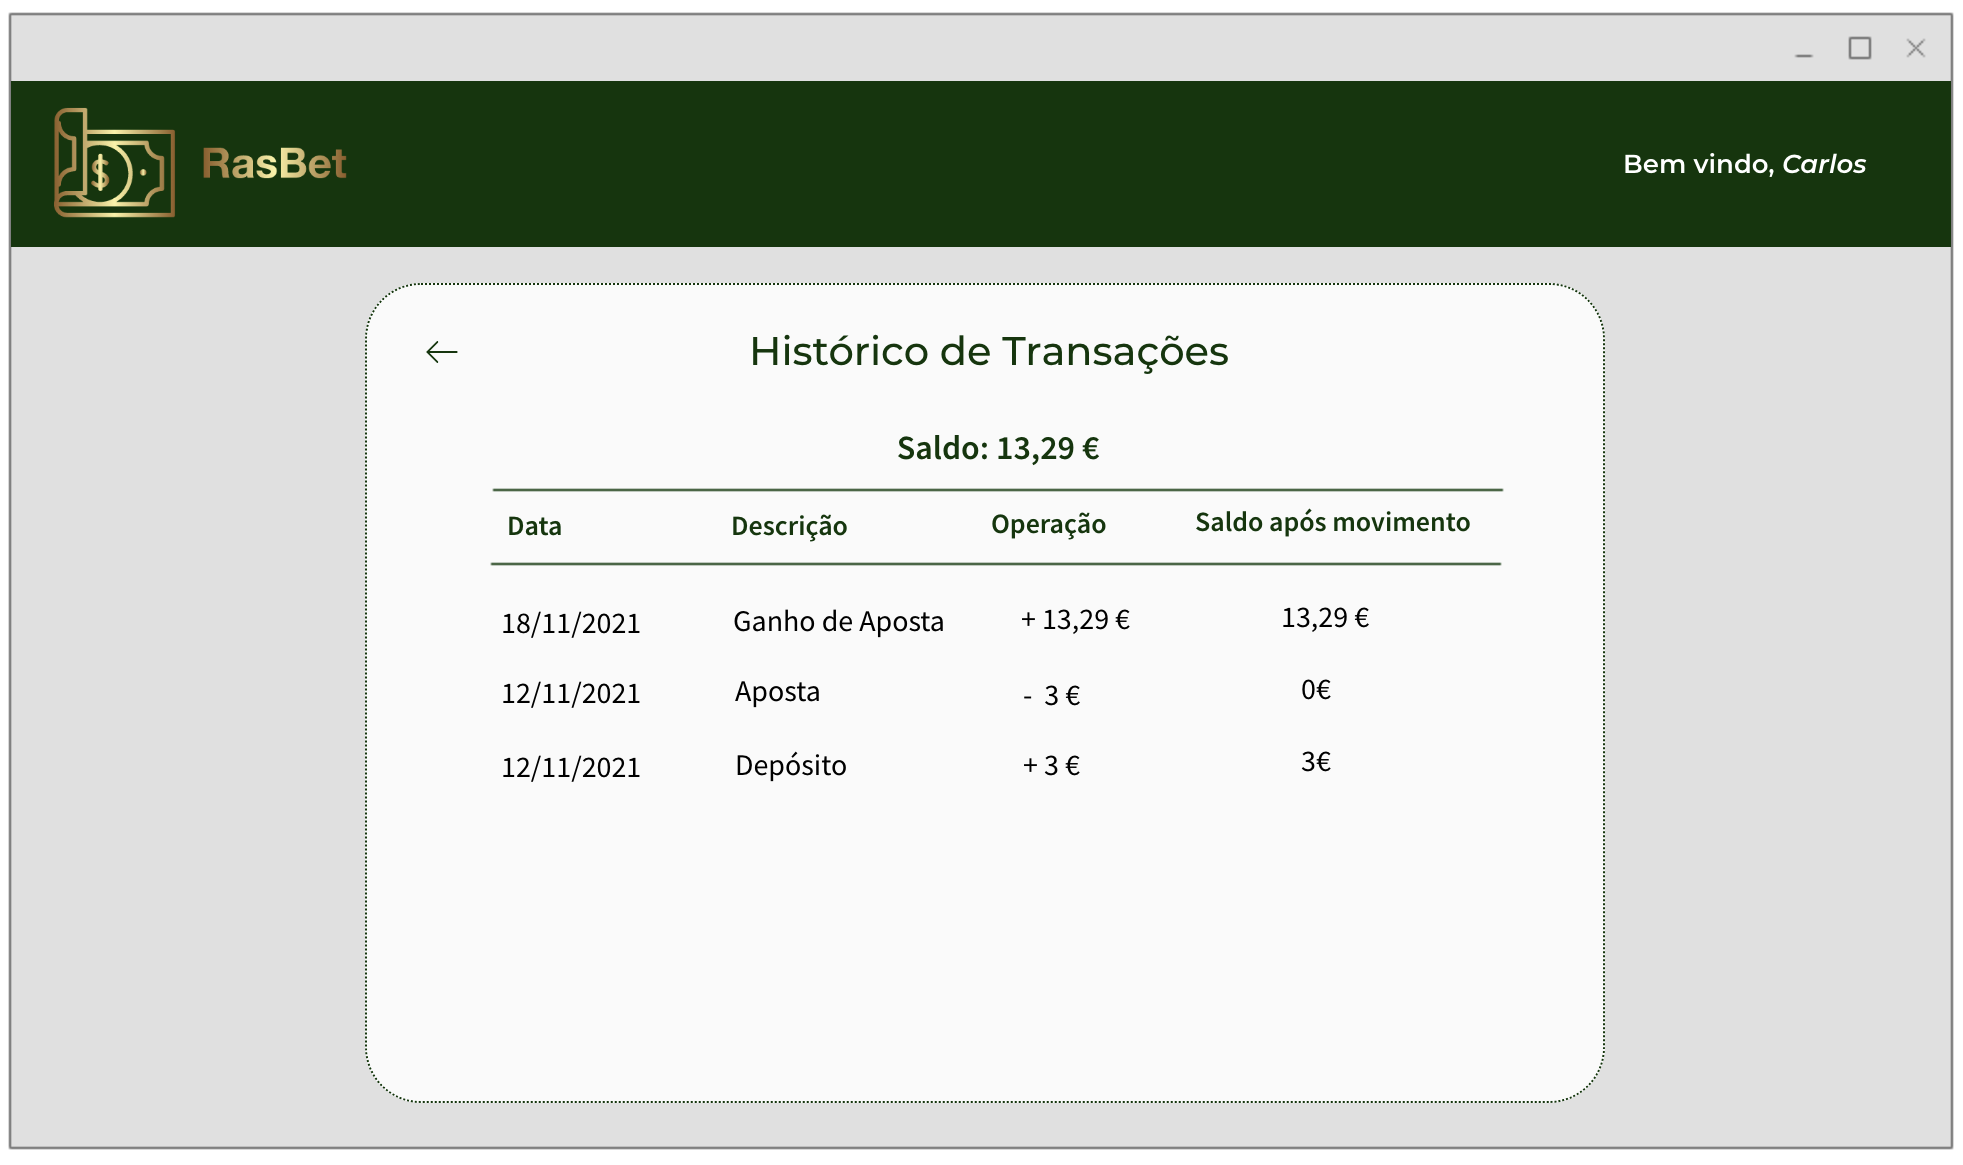
\includegraphics[width=1\textwidth]{imagens/ambitoProduto/Mockups/M_histTransacoes.png}
\caption{Mockup de Consultar histórico de Transações}
\end{figure}

\subsection{Depositar/Levantar dinheiro}
\begin{figure}[H]
\centering
\includegraphics[width=1\textwidth]{imagens/ambitoProduto/S_depositar:levantar.png}
\caption{Diagrama de Sequência de Depositar/Levantar dinheiro}
\end{figure}

\subsection{Inserir Odd}
\begin{figure}[H]
\centering
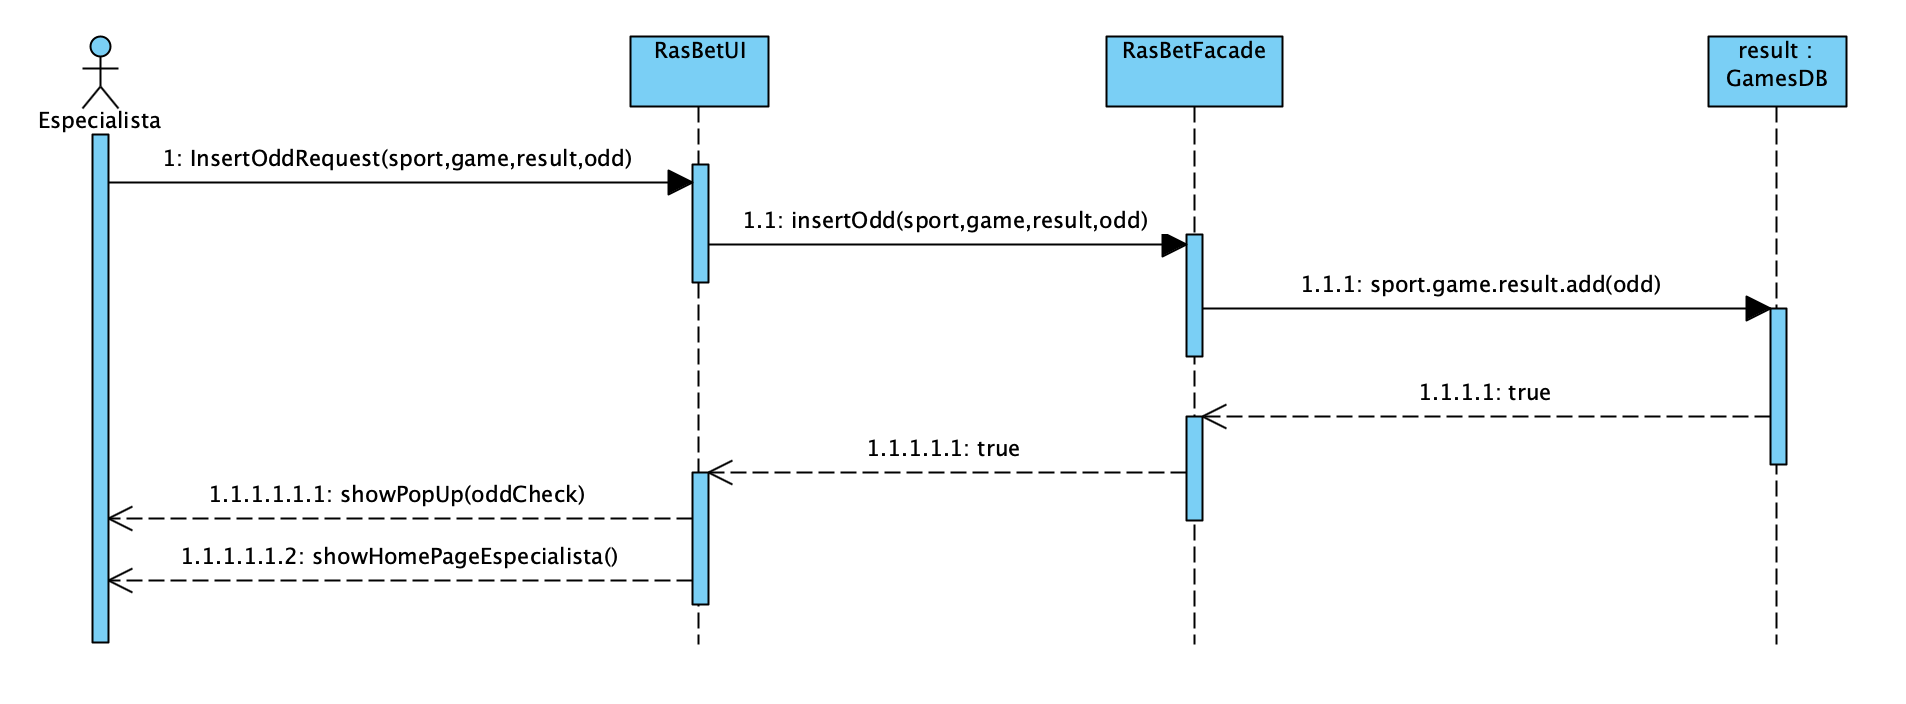
\includegraphics[width=1\textwidth]{imagens/ambitoProduto/SInserirOdd.png}
\caption{Diagrama de Sequência de Inserir Odd}
\end{figure}
\begin{figure}[H]
\centering
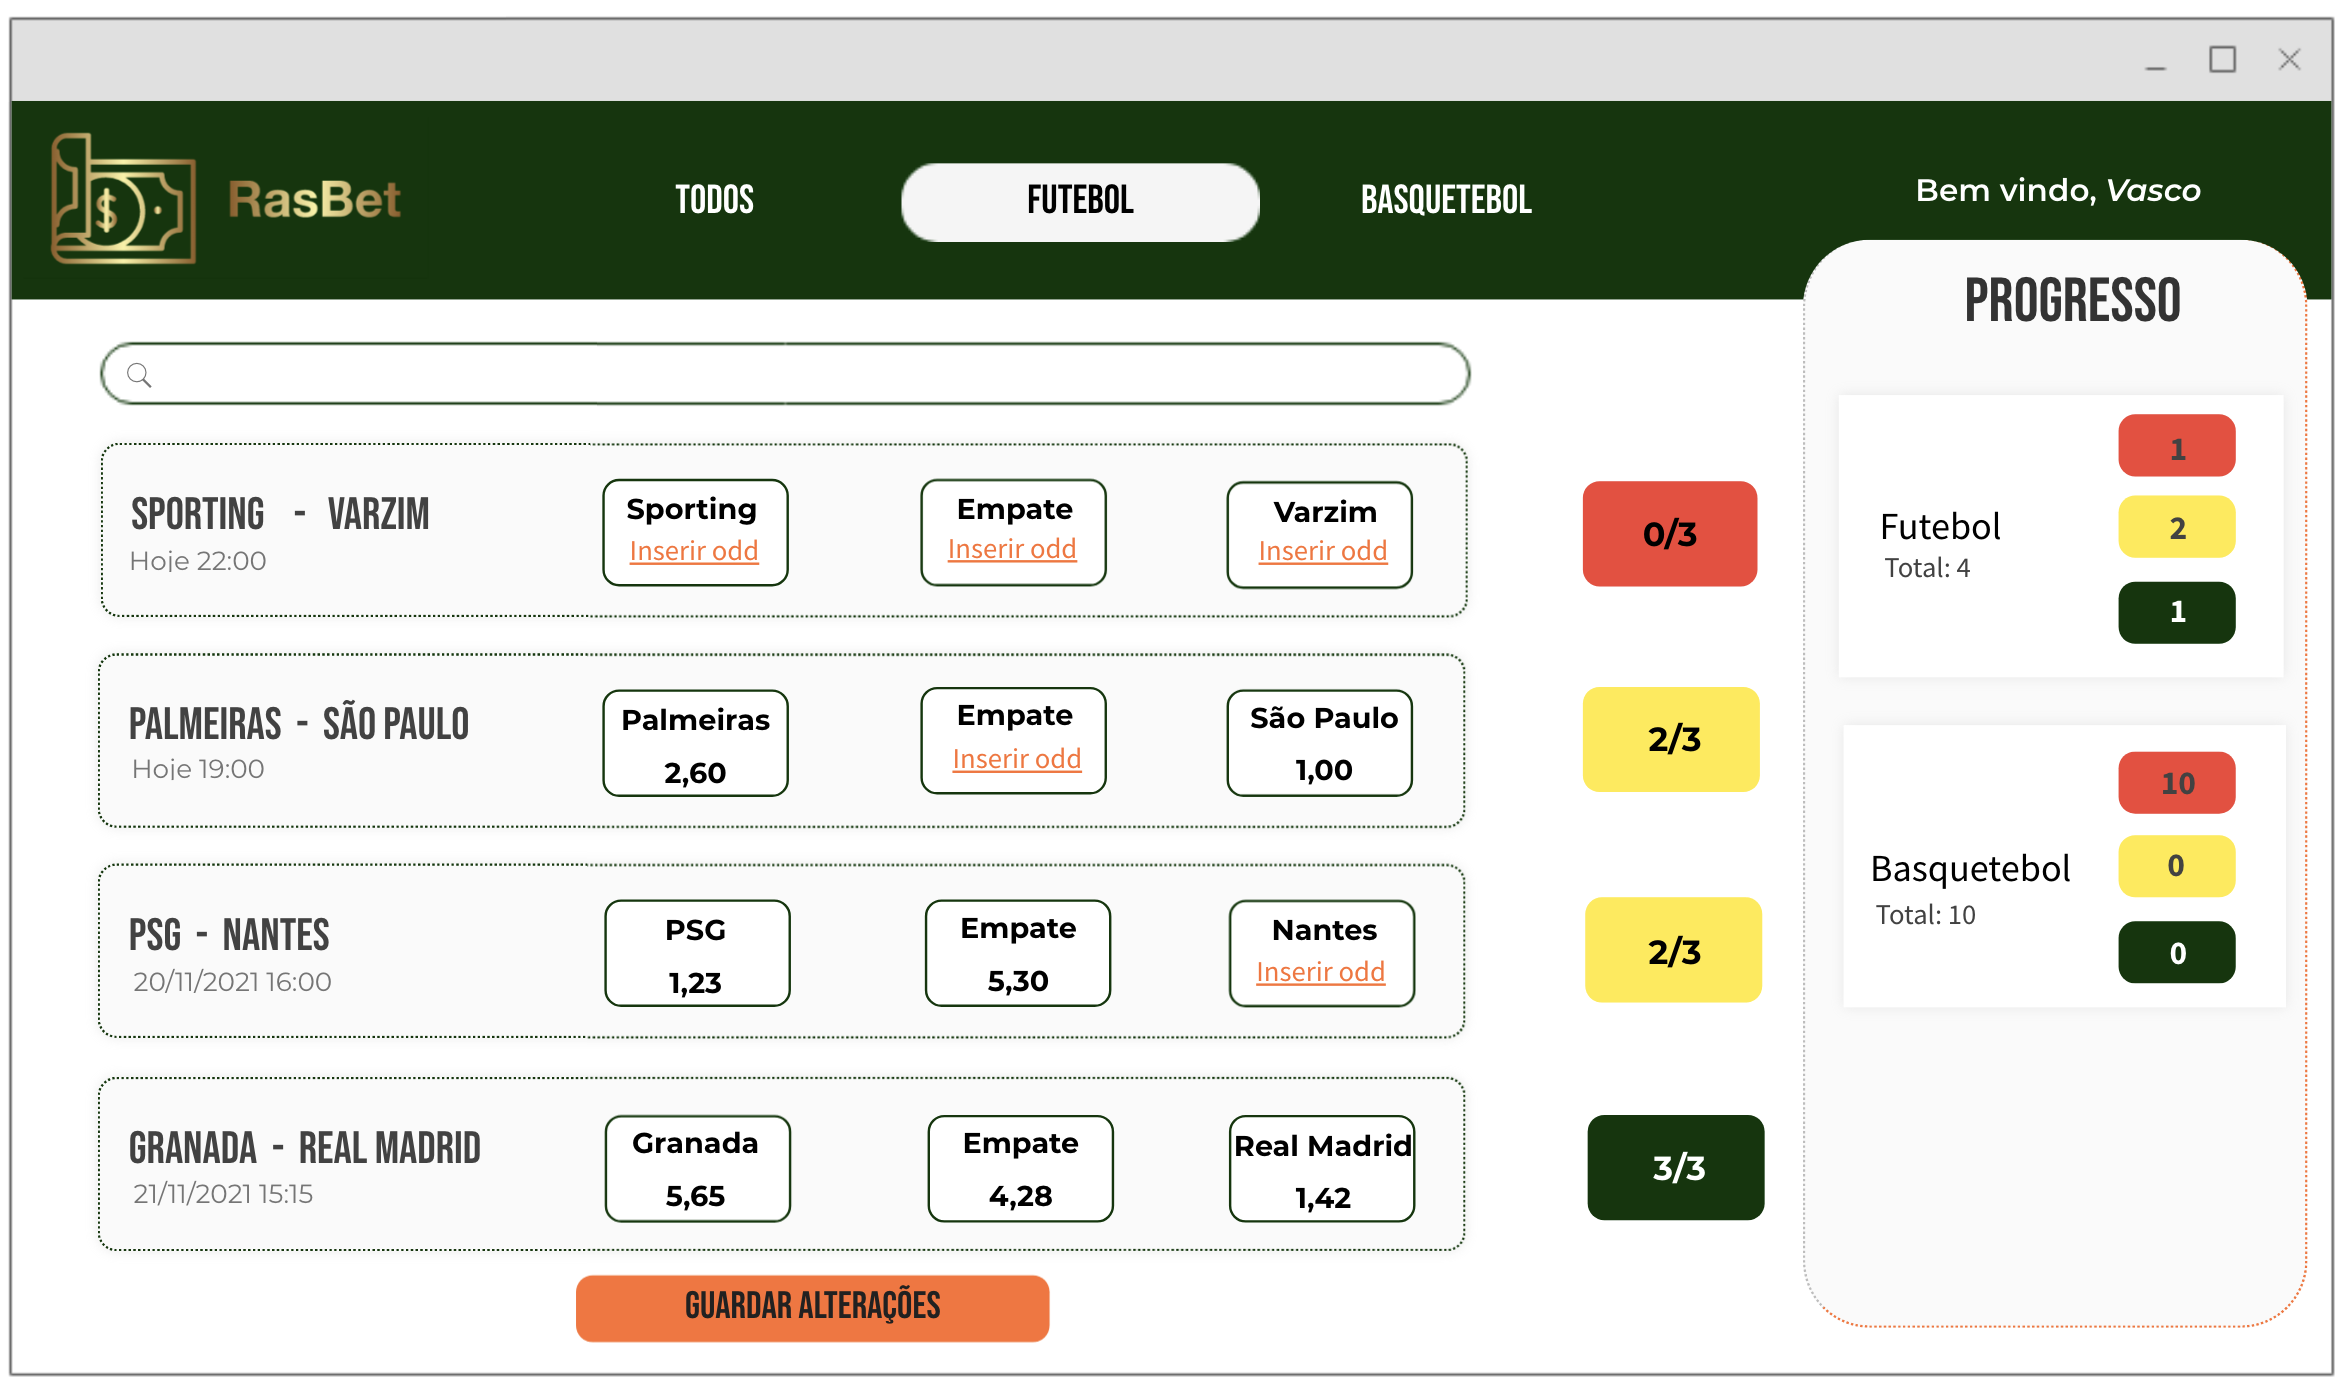
\includegraphics[width=1\textwidth]{imagens/ambitoProduto/Mockups/M_InserirODD.png}
\caption{Mockup de Inserir Odd}
\end{figure}

\subsection{Alterar e suspender jogos}
\begin{figure}[H]
\centering
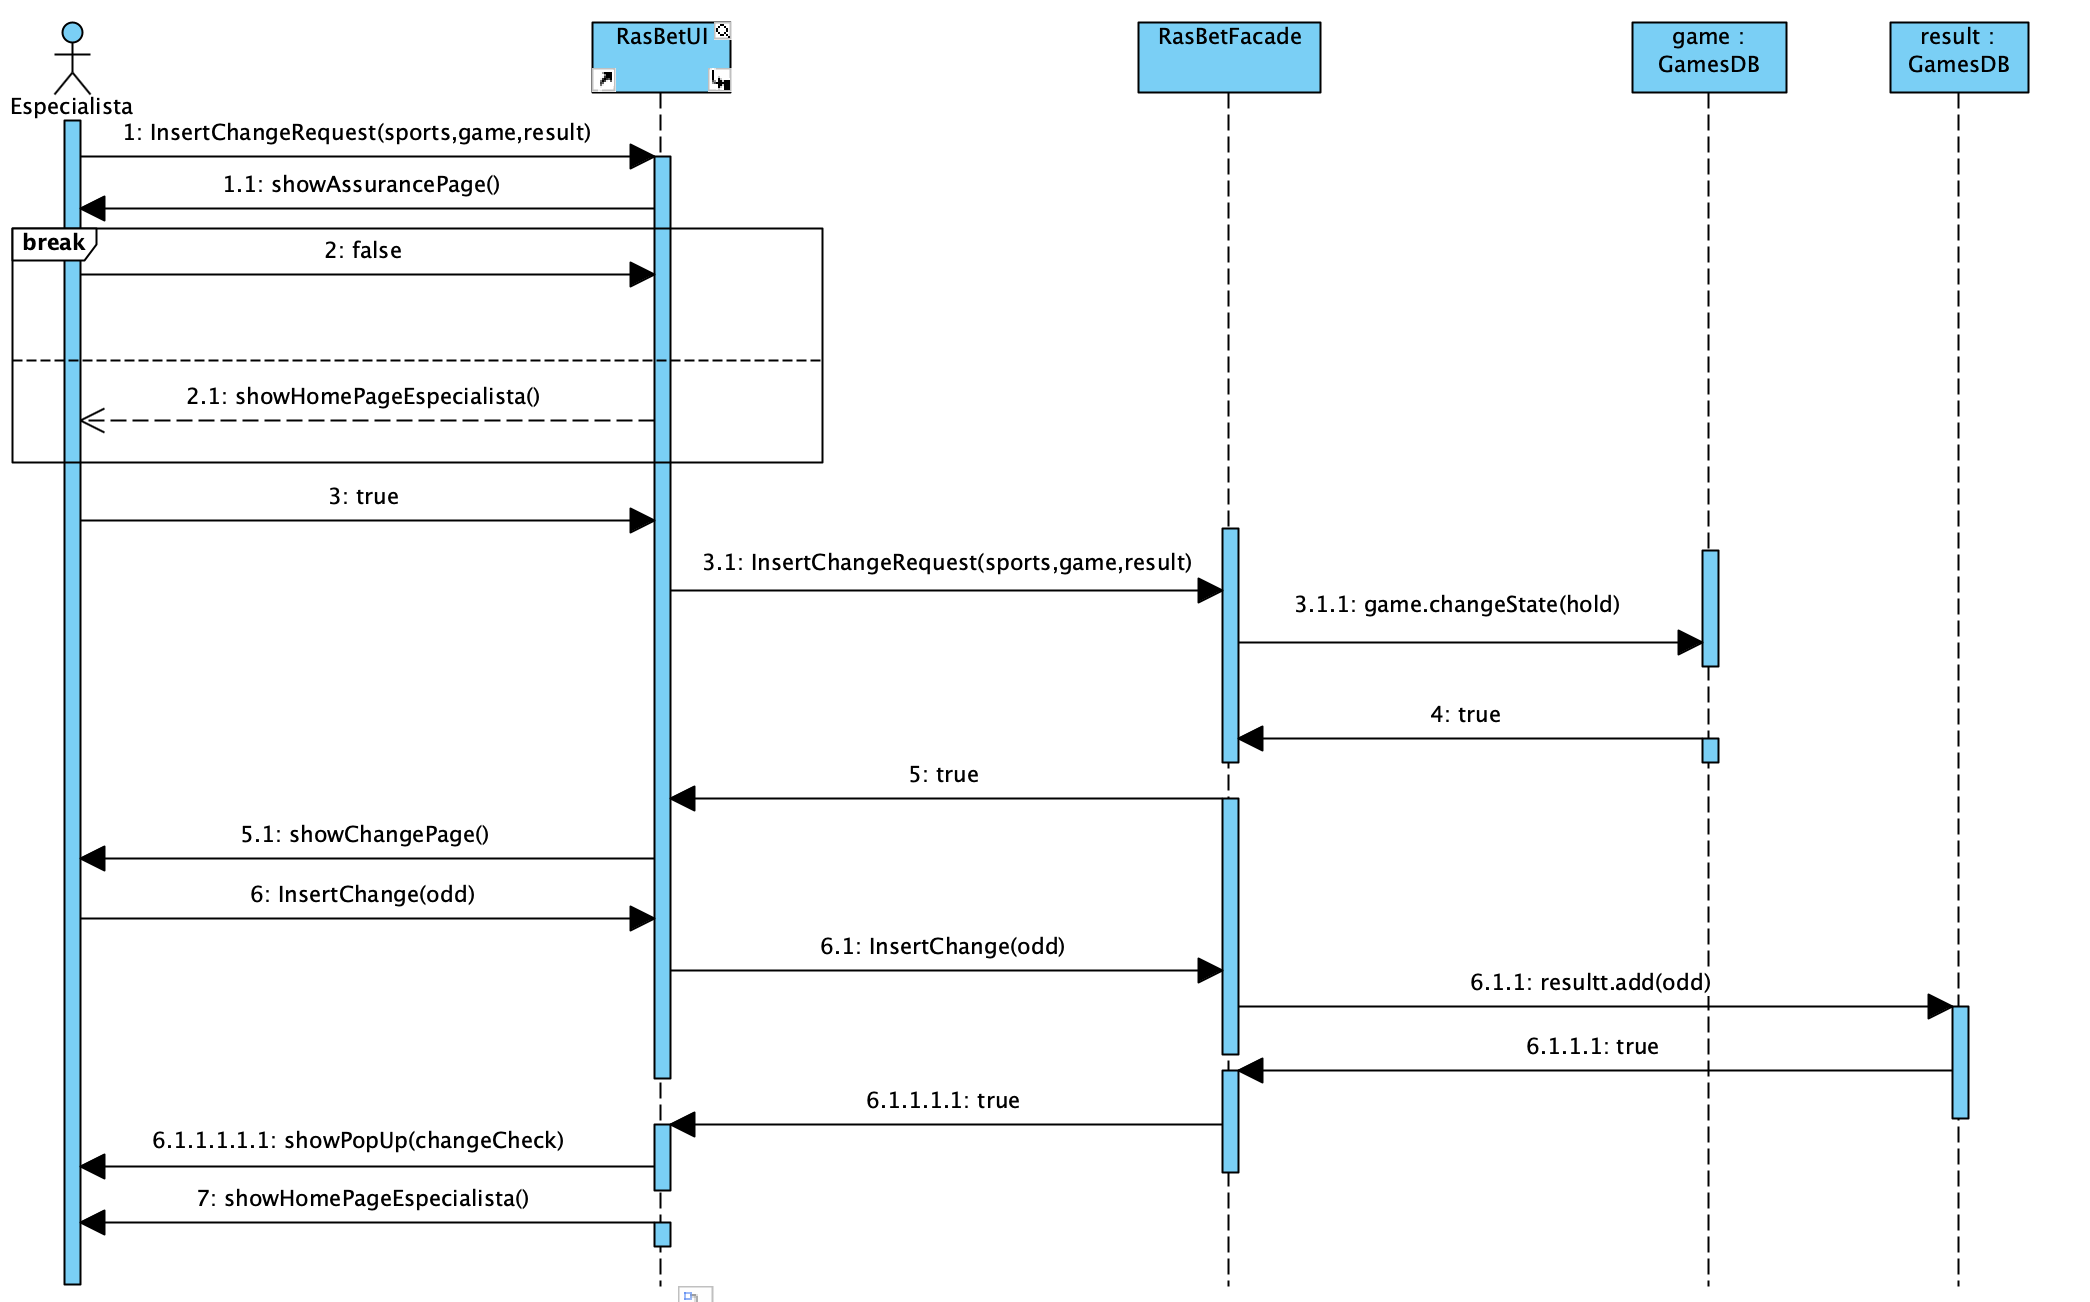
\includegraphics[width=1\textwidth]{imagens/ambitoProduto/S_alterar.png}
\caption{Diagrama de Sequência de Alterar e suspender jogos}
\end{figure}
\begin{figure}[H]
\centering
\includegraphics[width=1\textwidth]{imagens/ambitoProduto/Mockups/M_Altera:sus1.png}
\caption{Mockup de Alterar e suspender jogos 1}
\end{figure}
\begin{figure}[H]
\centering
\includegraphics[width=1\textwidth]{imagens/ambitoProduto/Mockups/M_Altera:sus2.png}
\caption{Mockup de Alterar e suspender jogos 2}
\end{figure}
\begin{figure}[H]
\centering
\includegraphics[width=1\textwidth]{imagens/ambitoProduto/Mockups/M_Altera:sus3.png}
\caption{Mockup de Alterar e suspender jogos 3}
\end{figure}